\documentclass[a4paper, 12pt]{book}
\usepackage[T1]{fontenc}
%\usepackage{bera}% optional: just to have a nice mono-spaced font
\usepackage{listings}
\usepackage{xcolor}
\usepackage{fancyhdr}
\usepackage{hyperref}
\colorlet{punct}{red!60!black}
\definecolor{delim}{RGB}{20,105,176}
\colorlet{numb}{magenta!60!black}
\definecolor{maroon}{cmyk}{0, 0.87, 0.68, 0.32}
\definecolor{halfgray}{gray}{0.55}
\definecolor{ipython_frame}{RGB}{207, 207, 207}
\definecolor{ipython_bg}{RGB}{247, 247, 247}
\definecolor{ipython_red}{RGB}{186, 33, 33}
\definecolor{ipython_green}{RGB}{0, 128, 0}
\definecolor{ipython_cyan}{RGB}{64, 128, 128}
\definecolor{ipython_purple}{RGB}{170, 34, 255}

\lstdefinelanguage{json}{
    stepnumber=1,
   	identifierstyle=\color{black}\ttfamily,
    numbersep=8pt,
    showstringspaces=false,
    breaklines=true,
    backgroundcolor=\color{ipython_bg},
    identifierstyle=\color{black}\ttfamily,
    commentstyle=\color{ipython_cyan}\ttfamily,
    stringstyle=\color{ipython_red}\ttfamily,
    keepspaces=true,
    showspaces=false,
    showstringspaces=false,
    rulecolor=\color{ipython_frame},
    frame=single,
    frameround={t}{t}{t}{t},
    framexleftmargin=5mm,
    numbers=left,
    numberstyle=\tiny\color{halfgray},
    % extendedchars=true,
    basicstyle=\scriptsize,
    keywordstyle=\color{ipython_green}\ttfamily,
    literate=
     *{0}{{{\color{numb}0}}}{1}
      {1}{{{\color{numb}1}}}{1}
      {2}{{{\color{numb}2}}}{1}
      {3}{{{\color{numb}3}}}{1}
      {4}{{{\color{numb}4}}}{1}
      {5}{{{\color{numb}5}}}{1}
      {6}{{{\color{numb}6}}}{1}
      {7}{{{\color{numb}7}}}{1}
      {8}{{{\color{numb}8}}}{1}
      {9}{{{\color{numb}9}}}{1}
      {:}{{{\color{punct}{:}}}}{1}
      {,}{{{\color{punct}{,}}}}{1}
      {\{}{{{\color{delim}{\{}}}}{1}
      {\}}{{{\color{delim}{\}}}}}{1}
      {[}{{{\color{delim}{[}}}}{1}
      {]}{{{\color{delim}{]}}}}{1},
}




\lstset{
    breaklines=true,
    extendedchars=true,
    literate=
    {á}{{\'a}}1 {é}{{\'e}}1 {í}{{\'i}}1 {ó}{{\'o}}1 {ú}{{\'u}}1
    {Á}{{\'A}}1 {É}{{\'E}}1 {Í}{{\'I}}1 {Ó}{{\'O}}1 {Ú}{{\'U}}1
    {à}{{\`a}}1 {è}{{\`e}}1 {ì}{{\`i}}1 {ò}{{\`o}}1 {ù}{{\`u}}1
    {À}{{\`A}}1 {È}{{\'E}}1 {Ì}{{\`I}}1 {Ò}{{\`O}}1 {Ù}{{\`U}}1
    {ä}{{\"a}}1 {ë}{{\"e}}1 {ï}{{\"i}}1 {ö}{{\"o}}1 {ü}{{\"u}}1
    {Ä}{{\"A}}1 {Ë}{{\"E}}1 {Ï}{{\"I}}1 {Ö}{{\"O}}1 {Ü}{{\"U}}1
    {â}{{\^a}}1 {ê}{{\^e}}1 {î}{{\^i}}1 {ô}{{\^o}}1 {û}{{\^u}}1
    {Â}{{\^A}}1 {Ê}{{\^E}}1 {Î}{{\^I}}1 {Ô}{{\^O}}1 {Û}{{\^U}}1
    {œ}{{\oe}}1 {Œ}{{\OE}}1 {æ}{{\ae}}1 {Æ}{{\AE}}1 {ß}{{\ss}}1
    {ç}{{\c c}}1 {Ç}{{\c C}}1 {ø}{{\o}}1 {å}{{\r a}}1 {Å}{{\r A}}1
    {€}{{\EUR}}1 {£}{{\pounds}}1
}

\lstdefinelanguage{python}{
    morekeywords={access,and,break,class,continue,def,del,elif,else,except,exec,finally,for,from,global,if,import,in,is,lambda,not,or,pass,print,raise,return,try,while},
    morekeywords=[2]{abs,all,any,basestring,bin,bool,bytearray,callable,chr,classmethod,cmp,compile,complex,delattr,dict,dir,divmod,enumerate,eval,execfile,file,filter,float,format,frozenset,getattr,globals,hasattr,hash,help,hex,id,input,int,isinstance,issubclass,iter,len,list,locals,long,map,max,memoryview,min,next,object,oct,open,ord,pow,property,range,raw_input,reduce,reload,repr,reversed,round,set,setattr,slice,sorted,staticmethod,str,sum,super,tuple,type,unichr,unicode,vars,xrange,zip,apply,buffer,coerce,intern},
    sensitive=true,
    morecomment=[l]\#,
    morestring=[b]',
    morestring=[b]",
    morestring=[s]{'''}{'''},
    morestring=[s]{"""}{"""},
    morestring=[s]{r'}{'},
    morestring=[s]{r"}{"},
    morestring=[s]{r'''}{'''},
    morestring=[s]{r"""}{"""},
    morestring=[s]{u'}{'},
    morestring=[s]{u"}{"},
    morestring=[s]{u'''}{'''},
    morestring=[s]{u"""}{"""},
    % {replace}{replacement}{lenght of replace}
    % *{-}{-}{1} will not replace in comments and so on
    literate=
    {á}{{\'a}}1 {é}{{\'e}}1 {í}{{\'i}}1 {ó}{{\'o}}1 {ú}{{\'u}}1
    {Á}{{\'A}}1 {É}{{\'E}}1 {Í}{{\'I}}1 {Ó}{{\'O}}1 {Ú}{{\'U}}1
    {à}{{\`a}}1 {è}{{\`e}}1 {ì}{{\`i}}1 {ò}{{\`o}}1 {ù}{{\`u}}1
    {À}{{\`A}}1 {È}{{\'E}}1 {Ì}{{\`I}}1 {Ò}{{\`O}}1 {Ù}{{\`U}}1
    {ä}{{\"a}}1 {ë}{{\"e}}1 {ï}{{\"i}}1 {ö}{{\"o}}1 {ü}{{\"u}}1
    {Ä}{{\"A}}1 {Ë}{{\"E}}1 {Ï}{{\"I}}1 {Ö}{{\"O}}1 {Ü}{{\"U}}1
    {â}{{\^a}}1 {ê}{{\^e}}1 {î}{{\^i}}1 {ô}{{\^o}}1 {û}{{\^u}}1
    {Â}{{\^A}}1 {Ê}{{\^E}}1 {Î}{{\^I}}1 {Ô}{{\^O}}1 {Û}{{\^U}}1
    {œ}{{\oe}}1 {Œ}{{\OE}}1 {æ}{{\ae}}1 {Æ}{{\AE}}1 {ß}{{\ss}}1
    {ç}{{\c c}}1 {Ç}{{\c C}}1 {ø}{{\o}}1 {å}{{\r a}}1 {Å}{{\r A}}1
    {€}{{\EUR}}1 {£}{{\pounds}}1
    %
    {^}{{{\color{ipython_purple}\^{}}}}1
    {=}{{{\color{ipython_purple}=}}}1
    %
    {+}{{{\color{ipython_purple}+}}}1
    {*}{{{\color{ipython_purple}$^\ast$}}}1
    {/}{{{\color{ipython_purple}/}}}1
    %
    {+=}{{{+=}}}1
    {-=}{{{-=}}}1
    {*=}{{{$^\ast$=}}}1
    {/=}{{{/=}}}1,
    literate=
    *{-}{{{\color{ipython_purple}-}}}1
     {?}{{{\color{ipython_purple}?}}}1,
    %
    identifierstyle=\color{black}\ttfamily,
    commentstyle=\color{ipython_cyan}\ttfamily,
    stringstyle=\color{ipython_red}\ttfamily,
    keepspaces=true,
    showspaces=false,
    showstringspaces=false,
    rulecolor=\color{ipython_frame},
    frame=single,
    frameround={t}{t}{t}{t},
    framexleftmargin=5mm,
    numbers=left,
    numberstyle=\tiny\color{halfgray},
    backgroundcolor=\color{ipython_bg},
    % extendedchars=true,
    basicstyle=\scriptsize,
    keywordstyle=\color{ipython_green}\ttfamily,
}
\usepackage[a4paper,top=3cm, bottom=3cm, inner=2.5cm, outer=2.5cm]{geometry}
\usepackage{times}
\usepackage[utf8]{inputenc}
\usepackage[spanish]{babel} % Comenta esta línea si tu memoria es en inglés
\usepackage{url}
%\usepackage[dvipdfm]{graphicx}
\usepackage{graphicx}
\usepackage{float}  %% H para posicionar figuras
\usepackage[nottoc, notlot, notlof, notindex]{tocbibind} %% Opciones de índice
\usepackage{latexsym}  %% Logo LaTeX
\usepackage{enumitem}

\title{Memoria del Proyecto}
\author{Santiago Carrión Vivanco}

\renewcommand{\baselinestretch}{1.5}  %% Interlineado

\begin{document}

\renewcommand{\refname}{Bibliografía}  %% Renombrando
\renewcommand{\appendixname}{Apéndice}

%%%%%%%%%%%%%%%%%%%%%%%%%%%%%%%%%%%%%%%%%%%%%%%%%%%%%%%%%%%%%%%%%%%%%%%%%%%%%%%%
% PORTADA

\begin{titlepage}
\begin{center}
\begin{tabular}[c]{c c}
%\includegraphics[bb=0 0 194 352, scale=0.25]{logo} &

\includegraphics[scale=0.25]{img/urjc_logo.jpg} &
\begin{tabular}[b]{l}
\Huge
\textsf{UNIVERSIDAD} \\
\Huge
\textsf{REY JUAN CARLOS} \\
\end{tabular}
\\
\end{tabular}

\vspace{3cm}

\Large
GRADO EN INGENIERÍA TELEMÁTICA

\vspace{0.4cm}

\large
Curso Académico 2017/2018

\vspace{0.8cm}

Trabajo Fin de Grado

\vspace{2.5cm}

\LARGE
SCRATCH4ROBOTS

\vspace{4cm}

\large
Autor : Santiago Carrión Vivanco \\
Tutor : Jose María Cañas Plaza
\end{center}
\end{titlepage}

\newpage
\mbox{}
\thispagestyle{empty} % para que no se enumere esta pagina

\maketitle

\cleardoublepage
%%%% \'indice de contenidos
\tableofcontents 
%%%% \'indice de figuras
\cleardoublepage
%\addcontentsline{toc}{chapter}{Lista de figuras} % para que aparezca en el indice de contenidos
\listoffigures % indice de figuras
%%%% \'indice de tablas
%\cleardoublepage
%\addcontentsline{toc}{chapter}{Lista de tablas} % para que aparezca en el indice de contenidos
%\listoftables % indice de tablas

\cleardoublepage
\pagestyle{plain}
\pagenumbering{arabic}
\chapter{Introducción}
\section{Robótica}
\label{sec:robotica}

La palabra Robot se deriva de la palabra de origen checoslovaco robota, que quiere decir siervo. Dicha palabra apareció por primera vez en la literatura en la obra R.U.R (1921)(Robot Universalis de Rossum), de Karel Capek.\\

Un robot es un sistema electromecánico que utiliza una serie de elementos hardware
(actuadores, sensores y procesadores) y cuyo comportamiento viene controlado por un
software programable que le da la inteligencia. La robótica se puede ver como la ciencia
y la tecnología de los robots, donde se combinan varias disciplinas como la mecánica, la
informática, la electrónica y la ingeniería artificial, que hacen posible el diseño hardware y software del robot.\\

Los robots se componen esencialmente de tres tipos de dispositivos: sensores,
procesadores y actuadores. En un robot los sensores son los encargados de recoger
la información del entorno. En este grupo se situarían: el láser, el sonar o las
cámaras. Estos dispositivos equivaldrían a nuestros sentidos humanos. Por otro lado se
encuentran los procesadores, encargados de analizar los datos que le son suministrados
por los sensores, también son los encargados de elaborar una respuesta a estos datos y
enviar la acción que deba llevarse a cabo a los actuadores, son como nuestro cerebro.
Por último los actuadores, principalmente motores eléctricos, se encargan de interactuar
con el entorno del mismo modo que lo hacen nuestros músculos.\\


\subsection{Historia}
\label{subsec:historia}

A finales del siglo XIX se presentan las primeras máquinas \textit{robots}, pero no
será hasta la segunda guerra mundial cuando se realicen los primeros diseños de esta
naturaleza.Con el desarrollo de las primeras computadoras digitales se produjo una
considerable evolución en este campo. Así, en 1970 una serie de investigadores del
Instituto de Investigación de Stanford desarrollaron Shakey (figura 1.1). Su sistema de
control creaba una reproducción interna del entorno a partir de los sensores de que
disponía y desde ella calculaba su movimiento.\\

Aunque es un termino relativamente nuevo y cuyo uso extendido es muy reciente, la historia lleva siglos dando pasos para llegar al punto en el que nos encontramos. Sin duda uno de los mayores impulsos en este mundo se produce con la llegada de la industrialización masiva. A principios de los 60, se instaló en una cadena de General Motors el primer robot industrial, Unimate, que realizaba tareas en la cadena de producción de los vehículos que podían ser peligrosas para los trabajadores.\\

En la misma década se creó el robot Shakey, el primero que combinó razonamiento lógico con acción física. Al igual que en el caso que trata este trabajo, Shakey utilizaba Planificación Automática para determinar sus acciones.\\

\begin{figure}[!htb]
	\begin{minipage}{0.48\textwidth}
    	\centering
     	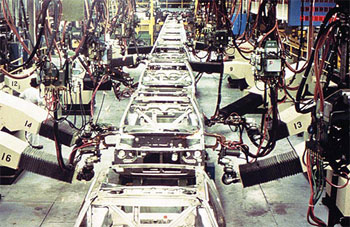
\includegraphics[scale=0.6]{img/unimate.jpg}
  		\caption{Unimate, General Motors}
  		\label{fig:unimate}
   	\end{minipage}\hfill
   	\begin {minipage}{0.48\textwidth}
     	\centering
     	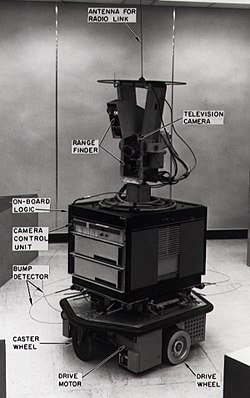
\includegraphics[scale=0.6]{img/shakey.jpg}
     	\caption{shakey en 1972}
     	\label{fig:shakey}
	\end{minipage}
\end{figure}

En 1970 se continua con la dinámica de crecimiento del sector, debido esta vez a la evolución del software ocurrida en esta época, y no parará hasta nuestros días, teniendo un crecimiento exponencial con una fuerte correlación con la evolución de software y hardware en general.
Desde este momento todas las grandes empresas dotaran sus fábricas de robots industriales. \\

En la actualidad uno de los mayores logros en el mundo de la robótica se da en 2011, la NASA lanzó al espacio el robot tipo vehículo explorador \textit{Curiosity} \ref{fig:curiosity} , que aterrizó en Marte al año siguiente. Su principal cometido es investigar la capacidad pasada y presente del planeta para alojar vida.\\

\begin{figure}[H]
    \centering
    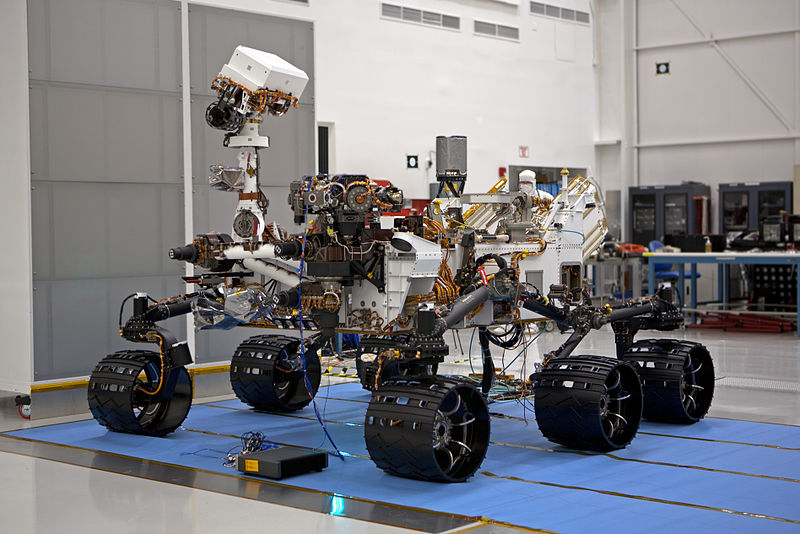
\includegraphics[scale=0.95]{img/curiosity.jpg}
  	\caption{El Curiosity en el Laboratorio de Propulsión a Chorro de la NASA}
  	\label{fig:curiosity}
\end{figure}

\subsection{Diferentes aplicaciones}
\label{subsec:diferentes aplicaciones}
Actualmente la robótica se encuentra en muchos ámbitos de nuestra vida cotidiana, algunas aplicaciones son:
\begin{itemize}
\item \textbf{Robótica educativa}: Es una disciplina que trabaja en la concepción creación e implementación de prototipos robóticos y programas con fines pedagógicos. Con ello se permite al alumno fabricar sus representaciones sobre los fenómenos del mundo, facilitar su adquisición y trasferencia a distintas áreas de conocimiento.
A través de la robótica educativa, los docentes pueden desarrollar de una forma práctica los conceptos teóricos que suelen ser abstractos y confusos, además despierta el interés del alumno por esos temas y relaciona al niño con el mundo tecnológico en el que se mueve. El empleo de un ambiente de aprendizaje basado en la robótica educativa ayuda al desarrollo de nuevas habilidades y conceptos, fortalece el pensamiento lógico, estructurado y formal del alumnado, desarrollando su capacidad para resolver problemas concretos.\\

Una de las características de este ámbito es la capacidad que posee para mantener la
atención del alumno, ya que manipula y experimenta haciendo que se concentre en sus
percepciones y observaciones sobre la actividad que realiza. Actualmente existen varios kits de robótica, algunos de ellos son: LEGO MINDSTORMS education, LEGO WeDo, LEGO NXT o Parallax Scribbler. Además, también existe la posibilidad de trabajar con programas con los que controlar y simular diferentes La robótica en Educación Infantil. Realidades y limitaciones robots como son NXT-G Educación, ROBOTC, ROBOLAB o Microsoft Robotics Developer Studio.

\item \textbf{Medicina}: Involucra en si varios ámbitos ya sea en cirugías de alto riesgo, en rehabilitaciones, en ayuda a personas con enfermedades de movilidad o discapacitados, en el almacenamiento de medicamentos y también en lo que se trata en pruebas ficticias y cirugías computarizadas.

\item \textbf{Militar}: La robótica donde más ha evolucionado es en la creación de vehículos autónomos, tecnología que tras unos años pasa a ser de uso civil.
Algunas de las creaciones que hemos heredado es el UAV, que se conocen comúnmente como dron, es una aeronave que vuela sin tripulación, Capaz de mantener de manera autónoma un nivel de vuelo controlado y sostenido, y propulsado por un motor de explosión, eléctrico, o de reacción.

\item \textbf{Robótica aeroespacial}: Uno de los mayores impulsores de la robótica ha sido la conquista del espacio, esta es una parte fundamental de la exploración espacial, debido a la imposibilidad de ser realizada en primera mano por un humano.
La idea básica sobre Robots Espaciales consiste en utilizar Inteligencia Artificial para
permitir a los robots realizar labores de exploración como si de un humano se tratase, desplazarse en terrenos y ambientes complejos de forma autónoma sin más conocimiento que lo recibido por sus sensores. Se busca no solo el proceso de pensamiento y análisis de los humanos en determinar las características del terreno, sino también la habilidad humana de conducir un vehículo en tiempo real.
\item \textbf{Industrial}: Las aplicaciones de la robótica industrial son cada vez mayores, algunos ejemplos son:
\begin{itemize}
\item Movimiento de material en almacenes: Un robot móvil es capaz de desplazarse por el almacén y recoger las unidades y referencias que incorporan un pedido concreto para un cliente.
\item Procesos de cadenas de montaje: Un robot antropomórfico es capaz de realizar movimientos complejos para colocar las distintas piezas que forman un producto final.
\item Empaquetado de producto: Tareas repetitivas y como puede ser el empaquetado de productos son realizadas por robots automatizados para hacer la misma tarea una y otra vez con alta velocidad y precisión, evitando errores y aumentando el ritmo de producción notablemente.
\item Procesos de alta precisión: Por ejemplo en la industria aeronáutica se utilizan cabezales de robots multifuncionales para el remachado en el fuselaje de un avión.
\item Seguimiento y verificación de productos: Un robot es capaz de realizar una evaluación al detalle del productor final, indicando si en el proceso de fabricación ha habido algún desperfecto o incorrección, estos robots suelen estar provistos de complejos sistemas de visión computacional.
\end{itemize}

\item \textbf{Automovilismo}: Los coches autónomos actualmente son una realidad, aún queda mucho desarrollo pero ya existen diversos modelos que se comercializan al público y conviven con el resto de automóviles. Esto es debido a la robustez que se ha conseguido en la lógica que gobierna estos coches. Se trata de uno de los retos cercanos más importantes de la robótica.\\
Para alcanzar una conducción realmente automática en una situación urbana con tráfico impredecible son necesarios muchos sistemas de tiempo real, que deben interoperar. Por ejemplo, es necesario un sistema de localización, de percepción del entorno, de planificación y lógicamente, un sistema de control. Además, son necesarios un conjunto de sensores que recojan y proporcionen la información necesaria para poder tomar las decisiones.

\item \textbf{Domótica}: Es el conjunto de tecnologías aplicadas al control y la automatización inteligente de la vivienda, que permite una gestión eficiente del uso de la energía, que aporta seguridad y confort, además de comunicación directa con los diferentes sistemas y elementos de una casa a través de la red.

Un sistema domótico es capaz de recoger información proveniente de unos sensores o entradas, procesarla y emitir órdenes a unos actuadores o salidas. El sistema puede acceder a redes exteriores de comunicación o información.
\end{itemize}

Es difícil no parase a pensar en la potencia que tiene esta rama de la ciencia y la
tecnología. Todo lo comentado deja claro la utilidad de esta área de desarrollo, que permitirá en el futuro ganar en comodidad, economía e incluso salud.

\subsection{Tipos de Robots}
\label{subsec:tipos de robots}

Ningún autor se pone de acuerdo en cuántos y cuáles son los tipos de robots y sus características esenciales. La más común son la que a continuación se presentan:

\textbf{Según su Estructura}:
\begin{itemize}
\item \textbf{Androides}: Un robot humanoide que se limita a imitar los actos y gestos de un humano, no es visto por el público como un verdadero androide, sino como una simple marioneta controlada por un humano. El androide siempre ha sido representado como una entidad que imita al ser humano tanto en apariencia, como en capacidad mental e iniciativa

\item \textbf{Poliarticulados}: En este grupo pueden encontrarse robots de diversas formas y configuraciones, pero su característica en común es la de ser sedentarios. Es decir, que son robots estructurados para moverse en un determinado espacio de trabajo, según uno o más sistemas de coordenadas y con un número limitado de grados de libertad.

\item \textbf{Móviles}: Estos robots cuentan con orugas, ruedas o patas que les permiten desplazarse de acuerdo a la programación a la que fueron sometidos. Estos robots cuentan con sistemas de sensores, que son los que captan la información que dichos robots elaboran. Los móviles son utilizados en instalaciones industriales, en la mayoría de los casos para transportar la mercadería en cadenas de producción así como también en almacenes. Además, son herramientas muy útiles para investigar zonas muy distantes o difíciles de acceder, es por eso que se suelen utilizar para realizar exploraciones espaciales o submarinas.

\item \textbf{Zoomórficos}: La locomoción de estos robots imita a la de distintos animales y se los puede dividir en caminadores y no caminadores. Estos últimos están aún muy poco desarrollados mientras que los caminadores sí lo están y resultan útiles para la exploración volcánica y espacial.

\item \textbf{Híbridos}: Este término corresponde a todos aquellos robots que son difíciles de clasificar, ya que corresponden a una combinación de las estructuras anteriormente explicadas. Por ejemplo, un robot híbrido, que esté conformado por la segmentación de articulaciones y ruedas, podría ser considerado tanto móvil, así como zoomórfico.

\end{itemize}

\begin{figure}[H]
	\begin{minipage}{0.48\textwidth}
    	\centering
     	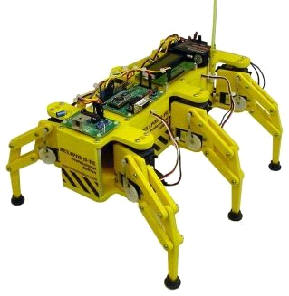
\includegraphics[scale=0.6]{img/robot-zoomorfico.jpg}
  		\caption{Robot zoomórfico}
  		\label{fig:zoomorfico}
   	\end{minipage}\hfill
   	\begin {minipage}{0.48\textwidth}
     	\centering
     	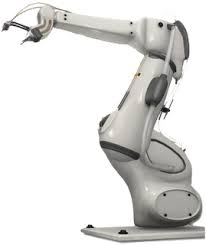
\includegraphics[scale=0.6]{img/robot-poliarticulado.jpg}
     	\caption{Robot poliarticulado}
     	\label{fig:poliarticulado}
	\end{minipage}
\end{figure}


\textbf{Según su Cronología}:
\begin{itemize}
\item \textbf{1ª Generación. Manipuladores}: Son sistemas mecánicos multifuncionales con un sencillo sistema de control, bien manual, de secuencia fija o de secuencia variable.

\item \textbf{2ª Generación. Robots de aprendizaje}: Repiten una secuencia de movimientos de movimientos que ha sido ejecutada previamente por un operador humano. El modo de hacerlo es a través de un dispositivo mecánico. El operador realiza los movimientos requeridos mientras el robot le sigue y los memoriza.

\item \textbf{3ª Generación. Robots con control sensorizado}: El controlador es una computadora que ejecuta las órdenes de un programa y las envía al manipulador para que realice los movimientos necesarios.

\item \textbf{4ª Generación. Robots inteligentes}: Son similares a los anteriores, pero además poseen sensores que envían información a la computadora de control sobre el estado del proceso. Esto permite una toma inteligente de decisiones y el control del proceso en tiempo real.
\end{itemize} 


\section{Software para robots}

Muchos robots poseen autonomía, la cual proviene del desarrollo de sistemas complejos, aplicaciones e infraestructuras que les dotan de inteligencia autónoma. El desarrollo de software robótico es similar al desarrollo de software en otros ámbitos, donde se parte de ciertos requisitos y se modela un diseño que será creado. Hace años el desarrollo de software robótico se realizaba adoptando soluciones ``ad hoc'', dotando a cada robot de un diseño específico, y con sensores y actuadores concretos. Esto suponía que no se podía aplicar el software desarrollado a otro robot, por lo que era necesario implementar de nuevo todo el software para un nuevo robot. En la actualidad, existen numerosas plataformas que permiten el desarrollo de aplicaciones robóticas de forma eficiente y genérica. Esto permite reutilizar gran parte de las aplicaciones creadas en otros robots, evitando el coste de realizar todo el proceso de nuevo.\\

Dotar al robot de cierta inteligencia conlleva desarrollar cierto software, el cual se suele programar apoyándose en herramientas, como los middleware robóticos, los simuladores robóticos, o las  bibliotecas que facilitan algunos aspectos. A continuación, se exponen algunas de estas herramientas que se emplean en la actualidad.\\

\subsection{Middlewares robóticos}

Actualmente existen diversos middlewares robóticos, con los que somos capaces de gestionar la complejidad y heterogeneidad del hardware y las aplicaciones, promover la integración de tecnologías en desarrollo, enmascarar los sistemas de percepción complejos, y simplificar el diseño de software.\\

Mediante el uso de middlewares somos capaces de introducir una capa de abstracción con los drivers y el hardware del robot, disminuyendo de manera importante la complejidad y los conocimientos necesarios para cualquier desarrollo. Además permite paralelizar de forma eficiente el trabajo.\\

\begin{figure}[H]
    	\centering
     	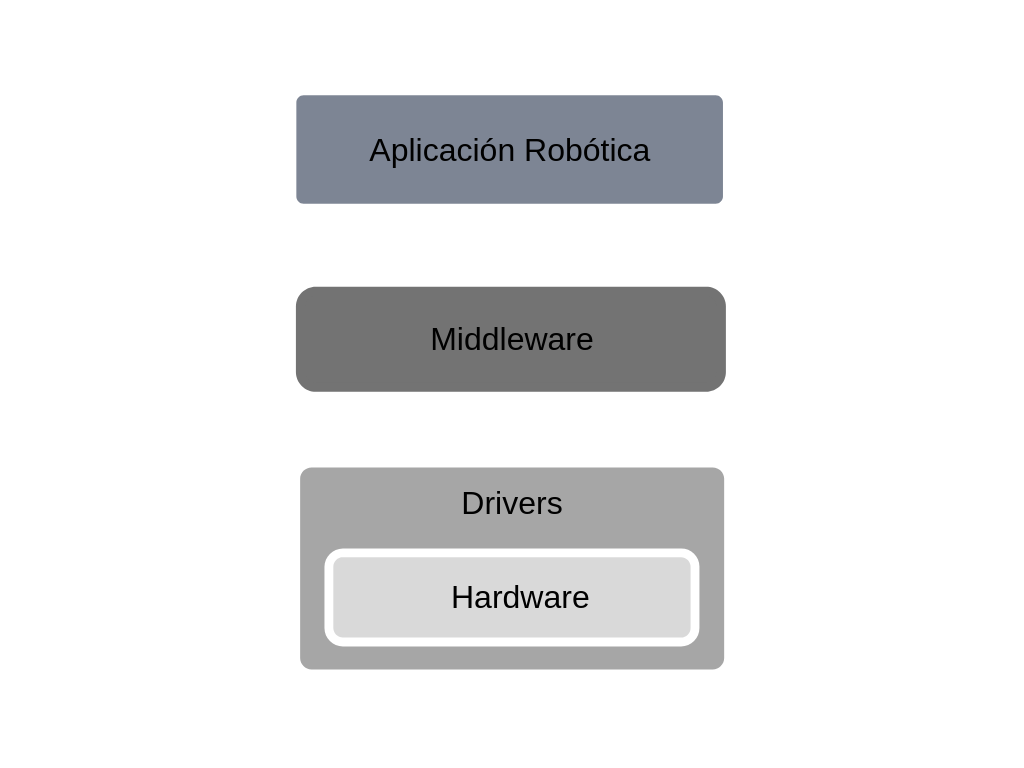
\includegraphics[scale=0.40]{img/middleware.png}
  		\caption{Esquema de capas en desarrollos de aplicaciones robóticas}
  		\label{fig:middleware}
\end{figure}

Algunos de los middlewares robóticos más destacados son:

\begin{itemize}
\item \textbf{ROS}\footnote{\url{http://www.ros.org/}}: Es una plataforma de software libre para el desarrollo de software de robots, que provee servicios estándar de un sistema operativo como la abstracción del hardware, el control de dispositivos de bajo nivel, mecanismos de intercambio de mensajes entre procesos y un conjunto de herramientas utilizadas ampliamente en robótica. La librería está orientada para un sistema UNIX, aunque se está adaptando a otros sistemas operativos como Fedora, Mac OS X, Arch, Gentoo, OpenSUSE, Slackware, Debian o Microsoft Windows, considerados como ``experimentales''.
En futuros capítulos hablaremos más en profundidad sobre ROS y su funcionamiento.

\item \textbf{ICE}\footnote{\url{https://zeroc.com/}}: Es un middleware de Código Abierto orientado a objetos que proporciona las herramientas, APIs y librerías necesarias para simplificar las comunicaciones entre componentes usando modelos basados en cliente y servidor y objectos distribuidos. Middleware usado para comunicación entre nodos, proporciona una capa transparente que se encarga de abrir y cerrar conexiones entre ellos, la serialización de la información a transmitir, además se encarga del manejo de perdidas de paquetes en estas transmisiones.

\item \textbf{Orocos}\footnote{\url{http://www.orocos.org}}: Es un proyecto de software libre para el control de robots y máquinas. Incluye cuatro bibliotecas C++: Real-Time Toolkit, Kinematics and Dynamics Library,  Bayesian Filtering Library y  Orocos Component Library. Está orientado a componentes, permitiendo añadir funcionalidades de forma sencilla y sin recompilar todo el código.  Incluye paquetes complementarios tales como Filtros de Bayes, Librerías de control Dinámico y Cinemático o Visión.

\item \textbf{Orca}\footnote{\url{http://orca-robotics.sourceforge.net/}}: Se trata de una plataforma de software libre para el desarrollo de aplicaciones robóticas. Fundamentalmente orientada al desarrollo de componentes, proporciona los medios para definir y desarrollar los componentes, los cuales pueden unirse para formar sistemas robóticos de distintas complejidades, desde vehículos autónomos hasta redes de sensores distribuidas.
Orca permite reutilizar código, de manera que se pueden emplear componentes robóticos ya creados.
\end{itemize}

\subsection{Simuladores robóticos}
El diseño de un robot es costoso y caro, lo que implica que muchos componentes necesarios para la construcción de los robots solamente estén disponibles para centros de investigación y corporaciones. Cuando se emplea un robot puede que el código desarrollado falle al probarlo, pudiendo incluso romperse algún robot.\\

Hoy en día existen numerosos simuladores robóticos, lo que permite a cualquier persona crear, programar y probar infinidad de robots de forma segura y económica. Algunos de los simuladores más empleados son:

\begin{itemize}
\item \textbf{Gazebo}\footnote{\url{http://gazebosim.org/}}: Es un simulador 3D de código abierto distribuido bajo licencia Apache 2.0. Este simulador se ha utilizado en ámbitos de investigación en robótica e Inteligencia Artificial. Contiene un potente motor de renderizado, soporta la incorporación de plugins lo que le hace ganar versatilidad, por ejemplo para integrarse middleware como ROS. Al ser muy popular y tener una gran comunidad se puede encontrar un amplio repertorio de robots comerciales.

\item \textbf{Stage}\footnote{\href{http://playerstage.sourceforge.net/index.php?src=stage}{stage}}: Simula robots móviles en el plano bidimensional y proporciona diversos tipos de sensores y actuadores. Su finalidad es ayudar a la investigación de sistemas autónomos de múltiples agentes, para lo cual proporciona gran cantidad de dispositivos simultáneamente.

\item \textbf{Webots}\footnote{\url{https://cyberbotics.com/}}: Es un simulador avanzado de robótica, que permite definir modelos propios, definir la física, escribir controladores para los robots y hacer simulaciones a gran velocidad. Se puede emplear en los sistemas operativos Linux, Windows y MacOS. Los lenguajes de programación que se pueden emplear son  C++, C y Java.
\end{itemize}

\subsection{Bibliotecas}
Las bibliotecas referidas al contexto de software son un conjunto de desarrollos que pueden ser usadas por terceros mediante una serie de interfaces bien definidas, que aportan de una funcionalidad añadida evitando tener que ser desarrollada desde un cero por el desarrollador que hace uso de ellas. Esto hace que agilicen y ayuden de forma notable cualquier proyecto, ya que únicamente debes centrarte en lo relativo a tu lógica, mientras que las cosas comunes puedes integrarlas en tu código a través de estas librerías.\\

Algunas de las bibliotecas utilizadas en robótica son:

\begin{itemize}
\item \textbf{OpenCV}\footnote{\url{https://opencv.org/}}: Es una biblioteca orientada principalmente a la visión computacional en tiempo real. La biblioteca es multiplataforma y gratuita para su uso bajo la licencia BSD de código abierto. Entre las áreas de aplicación de esta biblioteca destacan: segmentación y reconocimiento de objetos, reconocimiento de gestos, seguimiento del movimiento, estructura del movimiento,  y robots móviles.

\item \textbf{PCL}\footnote{\url{http://pointclouds.org/}}: Se utiliza para el procesamiento digital de imágenes RGBD mediante el tratamiento de nubes de puntos 3D. Contiene numerosos algoritmos de última generación que incluyen filtrado, estimación de características, reconstrucción de superficies, ajuste de modelos y segmentación entre otros. Para simplificar el desarrollo, PCL se divide en una serie de bibliotecas de código más pequeñas, que se pueden compilar por separado. Es multiplataforma y ha sido compilada con éxito en Linux, Mac OSX, Windows y Android / iOS.

\item \textbf{AForge.NET}\footnote{\url{http://www.aforgenet.com/}}: Es un framework C\# de código abierto diseñado para desarrolladores e investigadores en los campos de Visión por Computadora e Inteligencia Artificial. Sus áreas de aplicación son: procesamiento de imágenes, redes neuronales, algoritmos genéticos, lógica difusa, aprendizaje de máquinas, robótica, etc.
\end{itemize}

\section{Docencia en robótica}

Actualmente la robótica es un mercado al alza, esto hace que aumente de manera importante el número de científicos, ingenieros y técnicos demandados para trabajar e investigar en este sector.
Es importante una base sólida en conceptos de programación, procesado de imágenes, calculo, álgebra, electrónica, electricidad etc. Al ser un mundo complejo lleno de retos por resolver se necesita gente preparada, de ahí lo importante que es acercar a los más jóvenes desde los colegios e institutos a estas disciplinas.\\

Es por esto que la docencia en robótica intenta despertar el interés de los estudiantes transformando las asignaturas tradicionales en más atractivas e integradoras, ya que crea entornos de aprendizaje propicios que recrean los problemas del entorno que los rodea. En el futuro, tener nociones básicas de esta disciplina será clave debido a que cada vez de forma más habitual se implantan robots en diferentes sectores laborales.\\

La enseñanza en centros escolares principalmente se realiza mediante plataformas físicas como los robots LEGO (Mindstorms, NXT, Evo, WeDo), placas Arduino, los kits de SolidWorks, etc que con una simpleza espectacular son capaces de motivar al alumno ya que obtiene resultados vistosos y a los que le puede dar una aplicación en su vida cotidiana, despertando su interés en esta materia.\\
Otro sistema introducido en los últimos años en la educación es la programación de robots mediante lenguajes de programación visual, potentes lenguajes, que abstrayendo al alumno de la complejidad de la sintaxis, siendo muy intuitivos y dándole un entorno visual vistoso, hacen que estos software sean muy bien aceptados por los estudiantes de menor edad.\\

La capacidad de programar es una parte importante de la alfabetización en la sociedad actual. Cuando las personas aprenden a programar, aprenden estrategias importantes para resolver problemas, diseñar proyectos y comunicar ideas.

\section{Lenguajes de programación visual}
\label{sec:lenguajes}

Un lenguaje de programación visual es cualquier lenguaje de programación que permite a los usuarios crear programas manipulando elementos del programa gráficamente en lugar de especificarlos textualmente. Permite la programación con expresiones visuales y símbolos gráficos, utilizados como elementos de sintaxis o notación secundaria. Por ejemplo, muchos se basan en la idea de "cajas y flechas", donde las cajas u otros objetos de pantalla se tratan como entidades, conectadas por flechas, líneas o arcos que representan relaciones, mientras que otros se basan en el apilamiento de "cajas" con una función predefinida, creando así varios flujos de acciones programáticas con una objetivo final.\\

Estos lenguajes por regla general se usan en programación dirigida por eventos, La programación dirigida por eventos es un paradigma de programación en el que el flujo del programa está determinado por eventos o mensajes desde otros programas o hilos de ejecución.
Las aplicaciones desarrolladas con programación dirigida por eventos implementan un bucle principal o main loop donde se ejecutan las dos secciones principales de la aplicación: El selector de eventos y el manejador de eventos.\\

Podemos diferenciar varios niveles dentro de los lenguajes de programación visual:
\begin{itemize}
\item \textbf{Sintaxis}: En el nivel sintáctico, la explicación del bloque está limitada a estructura del lenguaje. Por ejemplo, una explicación podría revelar que una condición es parte de una declaración \textit{IF} y no debe ser confundido con una acción que se puede ejecutar en \textit{THEN} o \textit{ELSE} parte de una declaración. Sin embargo, este no trata de definir de forma específica qué es lo que define esa condición.
Intentan reducir o incluso eliminar por completo los errores sintácticos y ayudan a la creación de programas bien formados. Una analogía sería el corrector ortográfico en procesadores de texto que subraya o incluso corrige automáticamente palabras o gramática individuales.

\item \textbf{Semántica}: En el nivel de la semántica, se dan explicaciones sobre los bloques, a menudo implementadas a través de funciones de ayuda que describen el significado
de un bloque. El usuario obtiene una respuesta semántica en forma de panel de ayuda genérico incluyendo una breve descripción del significado del comando o bloque y la lista de opciones adicionales.

\item \textbf{Pragmática}: Permiten llevar nuestra implementación a un punto de testeo específico, nos ayudan con una serie de módulos propios a crear el entorno necesario para simular el funcionamiento de nuestro programa en ese estado.
\end{itemize}

\subsection{Motivación}
\label{subsec:motivacion}

Las principales motivaciones del uso de estos lenguajes son su \textbf{accesibilidad}, ya que no requiere de una infraestructura potente para su funcionamiento.
Además el \textbf{fácil aprendizaje} hace que sea un lenguaje idóneo para aquellos que no tienen ningún conocimiento de informática previo.
Y por último el eliminar de la ecuación algo tan simple como los \textbf{errores de sintaxis}, nos olvidamos completamente de este tipo de fallos, haciendo el desarrollo más fluido y menos frustrante para los principiantes, algo que puede marcar la diferencia a la hora de encontrar gratificante el desarrollo de aplicaciones con estos lenguajes.

\subsection{Ejemplos}
\label{subsec:tipos}

\begin{itemize}

\item \textbf{Scratch}\footnote{\url{https://scratch.mit.edu/}}: Es un proyecto del Grupo Lifelong Kindergarten del MIT Media Lab.
Es utilizado por estudiantes y docentes de todo el mundo para expresar ideas mediante animaciones, juegos e interacciones fácilmente programables con este entorno, hablaremos en capítulos siguientes más en profundidad de él.

\item \textbf{Blocly}\footnote{\url{https://developers.google.com/blockly/}}: El desarrollo de Blockly comenzó en el verano de 2011, y el primer lanzamiento público fue en Maker Faire en mayo de 2012. Blockly fue originalmente diseñado como un reemplazo para OpenBlocks en App Inventor. Es un proyecto de Google y es de código abierto. Por lo general, se ejecuta en un navegador web y se asemeja visualmente a Scratch. Blockly también se está implementando para Android e iOS aunque no todas las funciones basadas en el navegador web están disponibles para Android / iOS.
Utiliza bloques visuales que se unen entre sí para facilitar la escritura de códigos y generar código JavaScript, Python, PHP o Dart.

\begin{figure}[H]
    \centering
    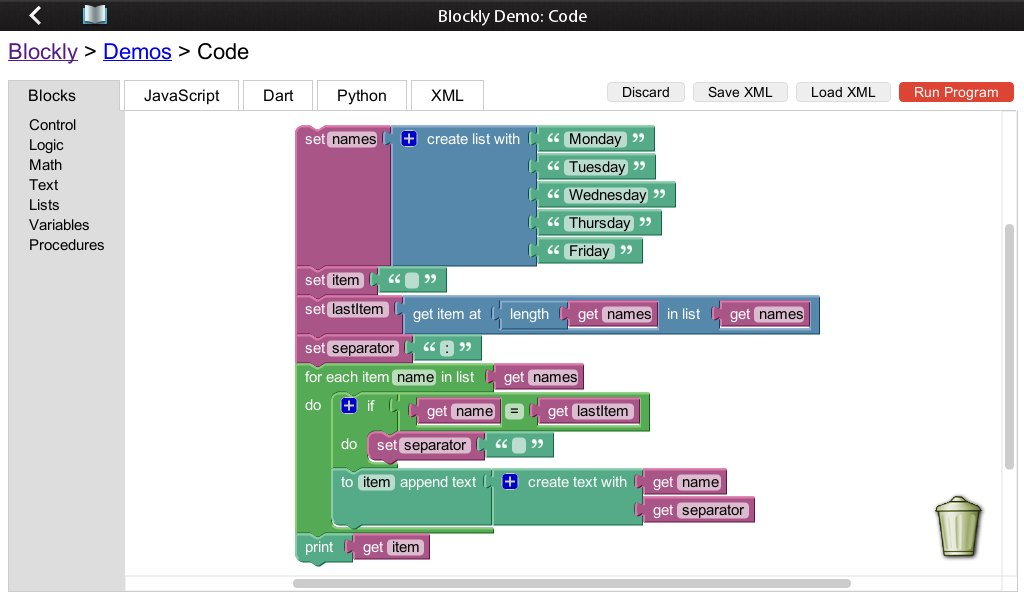
\includegraphics[scale=0.40]{img/blockly.jpg}
  	\caption{Lenguaje de programación visual Blockly}
  	\label{fig:blockly}
\end{figure}

\item \textbf{Snap!}\footnote{\url{https://snap.berkeley.edu/}}: Desarrollada por la Universidad de California en Berkeley, que sigue la filosofía de facilidad y sencillez para aprender a programar, Snap se basa en el conocido programa de Scratch, siendo su uso más extendido entre edades más maduras que las de Scratch.
Snap está programado en JavaScript. Esto hace que podamos usarlo desde cualquier navegador, ya sea desde un ordenador como desde las tablets.

\begin{figure}[H]
\centering
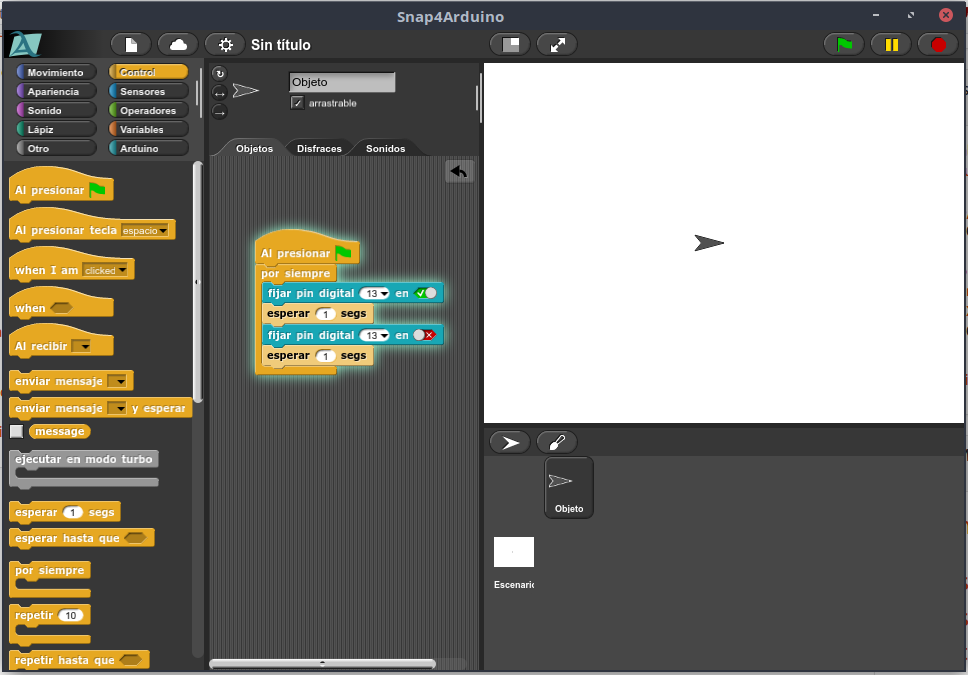
\includegraphics[scale=0.40]{img/snap.png}
\caption{Lenguaje de programación visual Snap!}
\label{fig:snap}
\end{figure}

\item \textbf{Kodu}\footnote{\url{https://www.kodugamelab.com/}}: Originalmente llamado Boku, es un entorno de desarrollo integrado de programación (IDE) de los laboratorios FUSE de Microsoft. El modelo de programación de Kodu está simplificado y puede programarse utilizando un controlador de juegos. Prescinde de la mayoría de las convenciones de programación que incluyen variables simbólicas, bucles, manipulación de números y cadenas, subrutinas, polimorfismo, etc.

Esta simplicidad se logra al ubicar la tarea de programación en un entorno de simulación ampliamente completo. El usuario programa los comportamientos de los personajes en un mundo 3d, y los programas se expresan en un paradigma sensorial de alto nivel que consiste en un sistema o lenguaje basado en reglas, basado en condiciones y acciones.

\begin{figure}[H]
\centering
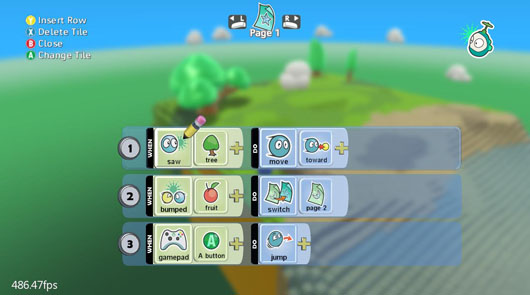
\includegraphics[scale=1]{img/kodu.jpg}
\caption{Lenguaje de programación visual Kodu}
\label{fig:kodu}
\end{figure}

\item \textbf{LEGO}: Lego dispone de una amplia gama de robots de aprendizaje programables (Mindstorms, NXT, Evo, WeDo), cada uno de estos robots de aprendijaze posee su propia sistema de programación, todos bajo interfaces gráficas fácilmente manipulables e intuitivas.\\
\begin{figure}[H]
	\begin{minipage}{0.48\textwidth}
    	\centering
     	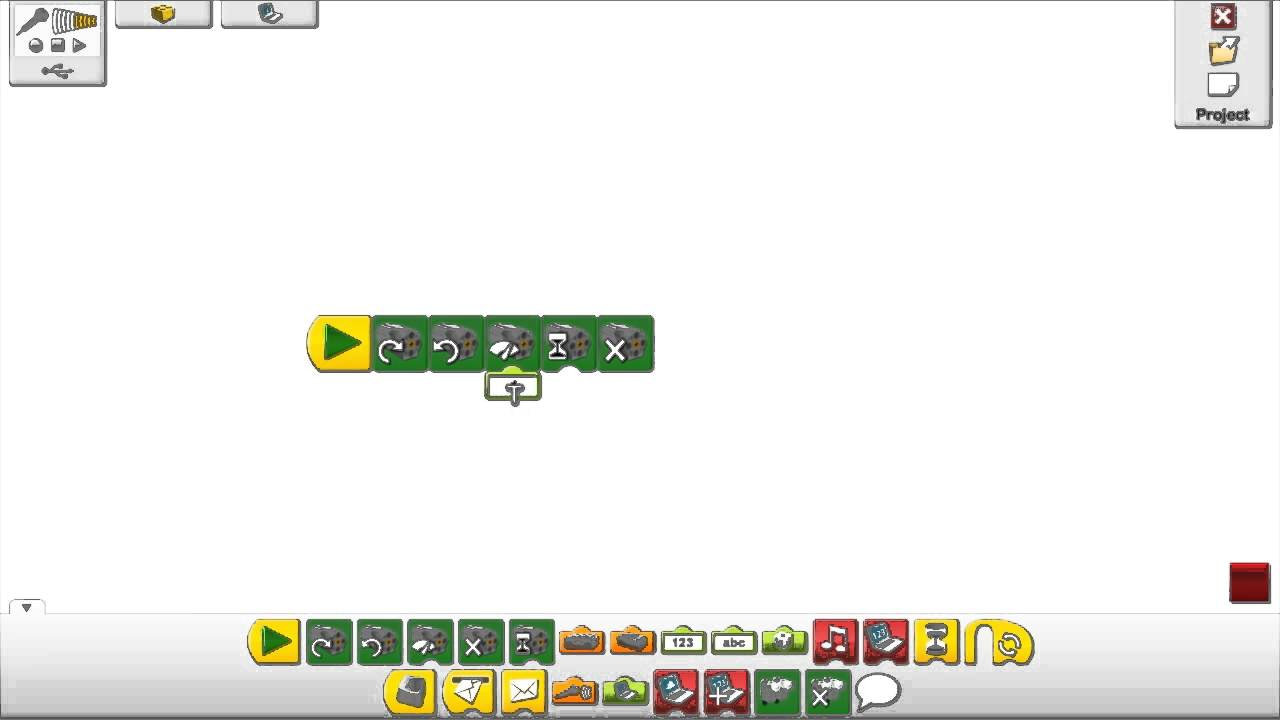
\includegraphics[scale=0.15]{img/lego-wedo.jpg}
  		\caption{Software de programación visual para LEGO WeDo}
  		\label{fig:lego-wedo}
   	\end{minipage}\hfill
   	\begin {minipage}{0.48\textwidth}
     	\centering
     	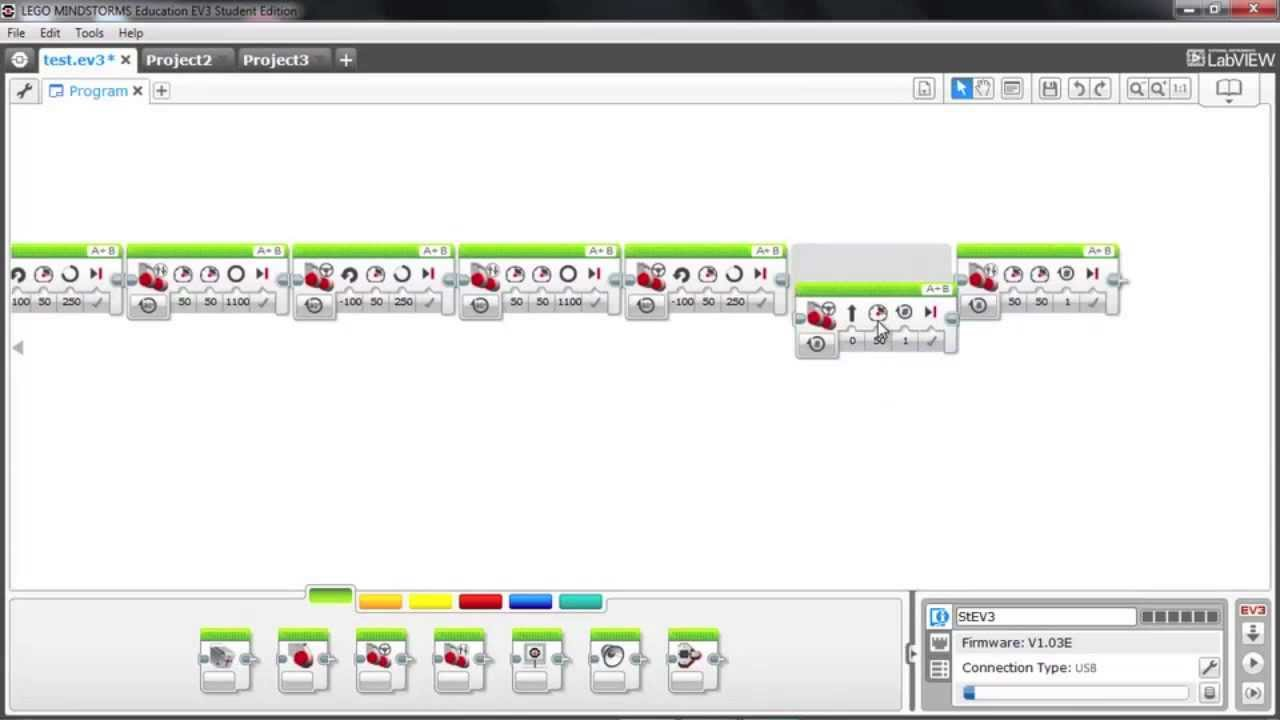
\includegraphics[scale=0.15]{img/lego-mindstorms.jpg}
     	\caption{Software de programación visual para LEGO Mindstroms}
     	\label{fig:lego-mindstorms}
	\end{minipage}
\end{figure}

\item \textbf{VisualStates}\footnote{\url{http://jderobot.org/VisualStates}}: Herramienta integrada en la suit de programación JdeRobot es una herramienta para la programación de comportamientos de robot utilizando máquinas de estados finitos de jerarquía (HFSM - Hierarchichal Finite State Machine). Representa gráficamente el comportamiento del robot en un esquema compuesto por estados y transiciones. Cuando el autómata está en cierto estado, pasará de un estado a otro según las condiciones establecidas en las transiciones. Esta representación gráfica permite un mayor nivel de abstracción para el usuario, ya que solo tiene que preocuparse por programar las acciones del robot y seleccionar qué componentes puede necesitar de la interfaz del robot.\\


\begin{figure}[H]
\centering
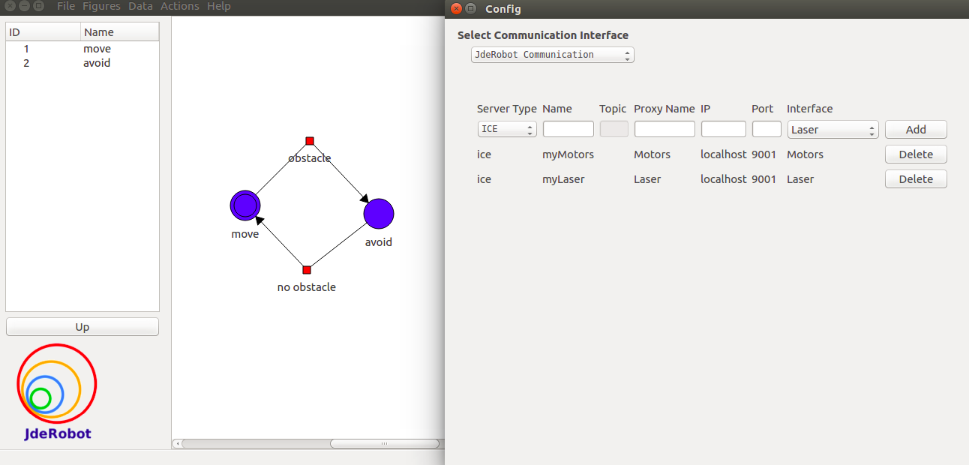
\includegraphics[scale=0.40]{img/visualstates.png}
\caption{Lenguaje de programación visual VisualStates}
\label{fig:visualstates}
\end{figure}

\item \textbf{Choregraphe}: Es el software de programación que permite a los usuarios crear y editar movimientos y comportamientos de NAO de manera sencilla. Su intuitiva interfaz gráfica, su biblioteca de comportamientos y las funciones de programación hacen posible realizar desde tareas simples como de nivel avanzado.

Es posible crear comportamientos utilizando la biblioteca de bloques de comportamiento con un simple arrastrar/copiar.
permite la programación basada en eventos, secuencial o en paralelo. Además la línea de tiempo permite programar por medio de secuencia lógica.

Los bloques de comportamiento pre-programadas son fácilmente configurables y con el editor de curvas o por medio de lenguaje Python.\\


\end{itemize}

\cleardoublepage
\chapter{Objetivos}
Tras haber expuesto las motivaciones y el contexto en el que se engloba este Trabajo de Fin de Grado, en este capítulo daremos una explicación más detallada del problema que se
intenta resolver.


\section{Descripción del problema}
\label{sec:descripcion del problema}
El propósito general es la mejora de la herramienta Scratch4Robots, que traduce programas en el lenguaje visual Scratch a programas en Python dentro del entorno ROS o del entorno JdeRobot. Como principales subobjetivos tenemos:
\begin{itemize}
\item \textbf{Mejora de la herramienta Scratch4Robots}:

Esta mejora la llevamos a cabo en la agregación de nuevos bloques visuales, y la refactorización de los ya existentes para aumentar las posibilidades y facilitar la usabilidad de la herramienta. Además buscamos acercar al usuario la herramienta con una documentación ajustada a usuarios con perfiles poco técnicos, acompañado de ejemplos didácticos.

\item \textbf{Generación de paquete ROS, para
facilitar su uso}:

Se va a publicar la herramienta en forma de paquete ROS, de forma que pueda ser instalable en cualquier máquina con un sistema operativo Ubuntu, y pueda acceder a sus funcionalidades a través de la consola de comandos, sin necesidad de descargar el código fuente de la herramienta. De esta forma evitamos que el usuario tenga que indagar en nuestro código fuente para tener que ejecutar nuestro nodo.

\item \textbf{Validación experimental con robots simulados}:

Buscamos exponer con forma de ejemplos prácticos, posibles casos de uso de la herramienta, de distintas complejidades.
\end{itemize}


\section{Requisitos}
\label{sec:requisitos}

Para cumplir los objetivos marcados de forma satisfactoria, debemos además satisfacer
los siguientes requisitos:

\begin{itemize}
\item El desarrollo deberá ser autocontenido en lo que sea posible, esto quiere decir que todas las librerías y dependencias de nuestra herramienta deberán estar contenidas en su interior. La programación se realizará en el
lenguaje Python.
\item El software desarrollado deberá ser compatible con Ubuntu 16.04, ROS-kinetic y Scratch 2.0 serán los únicos elementos indispensables para el correcto funcionamiento de nuestra herramienta.
\item Todos los componentes desarrollados deberán ser compatibles tanto trabajando en entornos simulados, como usando robots reales, esto se consigue usando todas las abstracciones de las que nos provee JdeRobot, y de todas las funcionalidades del middleware ROS.
\end{itemize}



\section{Metodología de trabajo}
\label{sec:metodologia}

Dada la naturaleza del proyecto, y al igual que en cualquier otro proyecto de software, es necesario el uso de un modelo que defina el ciclo de vida de la aplicación. Para el desarrollo de este proyecto hemos decidido adoptar el modelo de desarrollo en espiral.\\

El modelo en espiral consiste en una serie de ciclos que se repiten en forma de
bucle, cada ciclo representa un conjunto de actividades. Las actividades no están
prefijadas \textit{a priori}, sino que se eligen en función de las realizadas previamente. Estos ciclos se irán ejecutando hasta que la aplicación sea aceptada y no requiera otro
ciclo. Este modelo, definido por Barry Boehm en 1986, se basa en una espiral en la que cada iteración representa un conjunto de actividades.Estas actividades no tienen prioridad, se elegirá en la fase de análisis de riesgos. Así, cada iteración está dividida en las siguientes actividades:

\begin{itemize}
\item Determinar objetivos: en esta actividad se definirá el objetivo de la iteración actual. Siguiendo este modelo el objetivo final del proyecto se divide en subobjetivos, los cuales hemos definido anteriormente.
\item Análisis de riesgo: en esta actividad, se lleva a cabo varios estudios con el propósito de conocer las posibles amenazas o eventos no deseados que se puedan producir en el objetivo actual.
\item Desarrollar y probar: llegados a este punto será necesario la verificación del correcto funcionamiento realizado en la iteración para subsanar los errores y que estos no prosigan en las siguientes iteraciones. En este caso después de cada nuevo desarrollo se pasaba una batería de pruebas funcionales que aseguraban el funcionamiento de nuestra herramienta tras los nuevos desarrollos.
\item Planificación: en esta actividad se revisarán las fases anteriores para determinar si se debería continuar. En las reuniones semanales con el tutor se establecía la planificación y alcance de las siguientes actividades.
\end{itemize}

\begin{figure}[h]
    \centering
    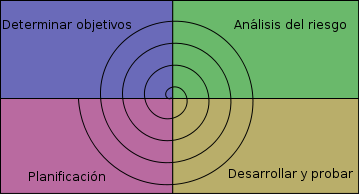
\includegraphics[width=0.75\textwidth]{img/metodologia_espiral}
    \caption{Desarrollo en espiral}
    \label{fig:espira}
\end{figure}

Para materializar estas actividades e iteraciones mantuvimos reuniones semanales con el tutor durante todo el desarrollo del trabajo. De este modo, cada semana marcábamos un nuevo subobjetivo. Si el anterior se había completado, planificábamos el siguiente. Si por el contrario, no sé había completado, ahondábamos en el objetivo actual para corregir los errores o volver a planificarlo.\\

Todo el código fuente generado se mantuvo en un repositorio Git\footnote{\url{https://github.com/JdeRobot/Scratch4Robots}}. De este modo el tutor y cualquier otra persona interesada tiene acceso en cualquier momento al código, además nos apoyamos del sistema de apertura de \textit{issues} en el repositorio remoto Git para cada implementación que se necesitaba desarrollar para la mejora del proyecto. De esta forma queda documentado todo el proceso de desarrollo de la herramienta.\\

Durante todo el desarrollo del trabajo se realiza un seguimiento de los objetivos a cumplimentar a través de una bitácora de trabajo\footnote{\url{http://jderobot.org/Scarrion-tfg}}.

\section{Plan de trabajo}
\label{sec:plan}

Simplificaremos la labor a desarrollar en este Trabajo de Fin de Grado en varios puntos:
\begin{itemize}
\item \textbf{Familiarización con el entorno software}: 

Como punto de partida, y durante el comienzo del trabajo nos centramos en la familiarización con el software que vamos a utilizar y desarrollar en un futuro. Estudamos JdeRobot, que es la plataforma de desarrollo principal utilizada en la mayoría de proyectos realizados en el departamento de robótica de la URJC. El objetivo principal de esta fase es aprender a utilizar este software, sus componentes y sus drivers para más adelante utilizarlos como parte de nuestro proyecto. Como parte del aprendizaje, se desarrolla una herramienta externa al core principal pero que usa de librerías y recursos de ella.\\

Además de JdeRobot, posteriormente nos centramos en ROS, que está muy presente en este trabajo, necesitando un conocimiento en profundidad de su arquitectura, su uso y de los componentes necesarios para desarrollar nuestro paquete propio basado en ROS.
\item \textbf{Estudio de Kurt y otras bibliotecas implicadas en la herramienta}: 

En un segundo periodo estudiaremos las bibliotecas implicadas en el funcionamiento interno de la herramienta, como punto fuerte de esta fase está el estudio de la biblioteca Kurt, que nos permite obtener toda la información necesaria de un proyecto Scratch, conocimiento de su API y su funcionamiento interno para saber qué podemos llegar a obtener y como usar esa información para proporcionar una traducción robusta al lenguaje Python.
\item \textbf{Mejora y desarrollo de nuevas funcionalidades}: 

Una vez entendido el software del que nos ayudamos para el desarrollo de la herramienta, es momento comenzar con la implementación de las mejoras. Aumentando el número de bloques robóticos propios que podremos usar en Scratch, esto es desarrollar la lógica detrás de cada bloque, todo programado en Python y la integración de estos bloques con Scratch. Dividimos los bloques entre bloques de uso genéricos, bloques aptos para drones y robots con ruedas. Estos bloques deben tener una funcionalidad muy específica y funcionar en armonía con el resto, tanto los propios de la aplicación Scratch como los nuevos bloques generados por nosotros propios de aplicaciones robóticas.
\item \textbf{Integración y documentación}: 

Una vez terminadas las mejoras de funcionalidades de la herramienta, nos centraremos en la mejora de su integración y uso.

Como objetivo tenemos la creación y publicación de nuestra herramienta como un paquete ROS, fácilmente instalable y ejecutable en cualquier entorno Ubuntu.

Con la documentación buscamos hacer la herramienta lo más intuitiva posible, mejorando scripts de lanzamiento y de generación de código. Creando ejemplos autocontenidos para una rápida demostración de la potencia de la herramienta y generando tutoriales tanto escritos como con vídeo para evitar confusiones.
\item \textbf{Validación Experimental}:

Por último buscamos la validación del funcionamiento de la herramienta, desarrollando ejemplos de distintas complejidades.
\end{itemize}


\cleardoublepage
\chapter{Infraestructura}
\section{Scratch}
\label{sec:scratch}

Scratch es un proyecto del Grupo Lifelong Kindergarten del MIT Media Lab.
Es utilizado por estudiantes y docentes de todo el mundo para expresar ideas mediante animaciones, juegos e interacciones facilmente programables con este entorno.

El nombre proviene de la palbra \textit{scratching} que en el mundo de la informática se refiere a reutilizar código, el cual puede ser usado de forma beneficiosa y efectiva para otros propósitos y fácilmente combinado, compartido y adaptado a nuevos escenarios, lo cual es una característica clave de Scratch.

Es la segunda versión principal actual de Scratch, siguiendo a Scratch 1.4. Cuenta con un editor y un sitio web rediseñados, y permite al usuario editar proyectos directamente desde su navegador web, así como en un editor fuera de línea.

Se lanzó oficialmente en 2013 y ha sido completamente reescrito en Adobe Flash además debido a las nuevas características y al diferente lenguaje de programación, los proyectos de Scratch 2.0 se guardan en formato .sb2.

Scratch se define por una interfaz intuitiva y de simple manejo compuesta por tres zonas claramente diferenciadas. En la zona izquierda tendremos un escenario y un selector de \textit{sprites}, en el centro encontramos las diferentes categorías de bloques que podemos utilizar y un listado de los bloques pertenecientes a la categoría seleccionada, y por último tendremos un espacio vacio en la parte derecha en la que crearemos nuestro proyecto, con el simple movimiento de arrastrar el bloque deseado.

Tendremos bloques de las siguientes categorias:
\begin{itemize}
\item \textbf{Movimiento}: Mueve objetos y cambia ángulos.	  	 	
\item \textbf{Eventos}: Contiene manejadores de eventos situado al principio de cada grupo de instrucciones.
\item \textbf{Apariencia}: Controla el aspecto visual del objeto, añade bocadillos de habla o 
pensamiento, cambia el fondo, ampliar o reducir.	 	
\item \textbf{Control}: Sentencian condicionales.
\item \textbf{Sonido}: Reproduce ficheros de audio y secuencias programables.	 	
\item \textbf{Sensore}: Los objetos pueden interactuar con el ambiente que ha creado el usuario.
\item \textbf{Lápiz}: Control del ancho, color e intensidad del lápiz.	 	
\item \textbf{Operadores} Operadores matemáticos, generador aleatorio de números, operadores booleanos.
\item \textbf{Datos}: Creación de variables y listas.	 	
\item \textbf{Mas Bloques}: Dispositivos o bloques externos creados por el usuario.
\end{itemize}

Al ser una herramienta madura y muy extendida existe una gran comunidad con la que compartir y de la que obtenter proyectos.

\begin{figure}[H]
    \centering
    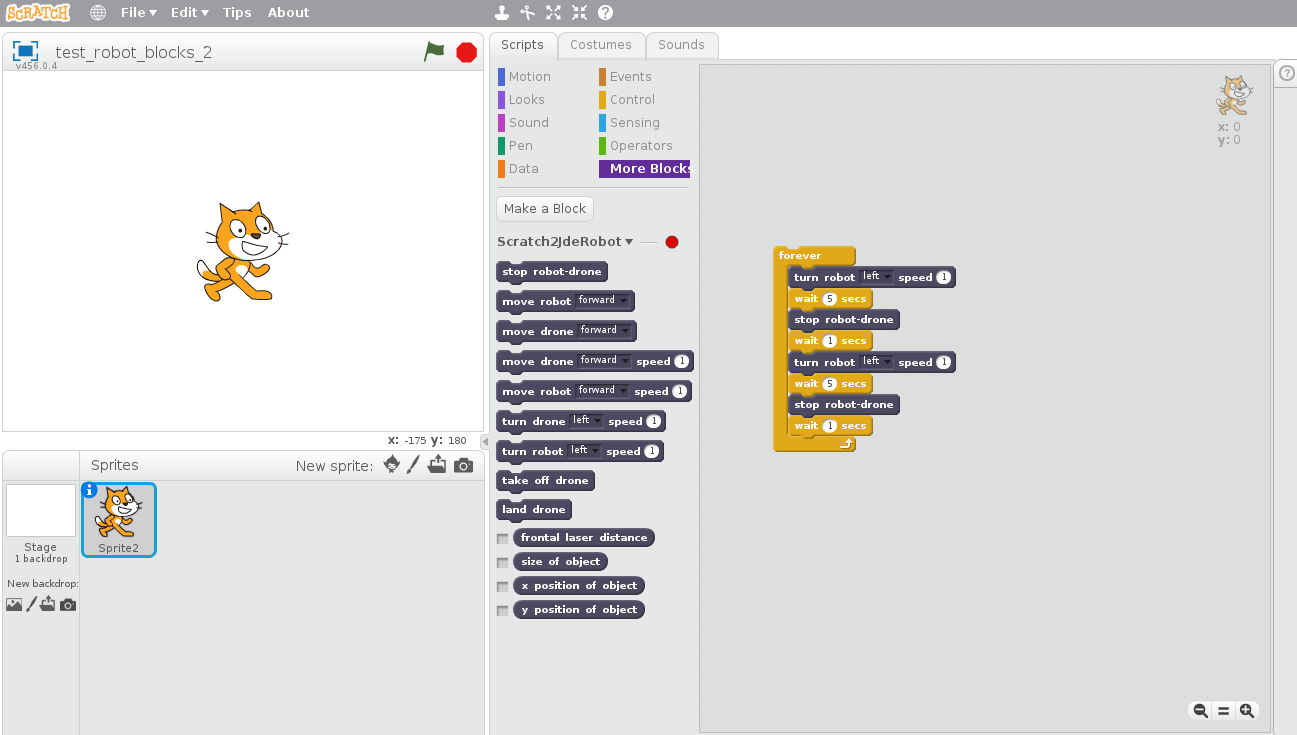
\includegraphics[scale=0.32]{img/scratch_IDE.png}
  	\caption{Espacio de trabajo de Scratch 2.0}
  	\label{fig:gazebo}
\end{figure}

\section{JdeRobot}
\label{sec:jderobot}

Nace de la tesis doctoral de Jose María Cañas en el año 2003 llevando desde ese momento en continua evolución y desarrollo, adaptandose a las tecnologías del momento.
Es una suite de desarrollo de software de robótica, domótica y sistemas de
visión computerizados cuya última versión, la 5.6, es la usada en este proyecto y permite la integración con ROS Kinetic. Proporciona un entorno distribuido donde las aplicaciones se forman mediante una colección de componentes asíncronos concurrentes, que se conectan mediante el middleware de comunicación ICE o mensajes ROS.
Se compone de interfaces, drivers, utilidades y aplicaciones para el desarrollo de cualquier proyecto de robótica
En este proyecto nos ayudamos de librerías como pueden ser \textit{comm, Config, JdeRobotTypes} que nos ayudan a agilizar el desarrollo de nuestra herramienta, abstraernos de ciertos niveles de complejidad y hacemos uso de una cantidad de entornos simulados en Gazebo con los que probar el correcto funcionamiento.


\section{Librería Comm}
\label{sec:libreria-com}

Librería desarrollada por JdeRobot con versiones tanto en python como en C que nos abstrae del tipo de comunicación utilizada por nuestros componentes.
Apoyandose en las librerías ya definidas en JdeRobot para el fácil uso de nodos ROS y Ice crea una capa de abstracción que permite que una aplicación sea capaz de funcionar tanto con \textit{ROS} como con comunicación \textit{Ice} sin necesidad de modificar el código interno de esta. De esta forma se aprovecha el trabajo anterior, se economiza tiempo, y se reduce el código redundante.
Su funcionamiento se apoya en el uso de un fichero de configuración necesario para establecer el tipo de comunicación que usaran los sensores y actuadores de nuestro robot. De este fichero obtendremos el tipo de comunicación y toda la información necesaria para poder establecerla. 
Se trata de un paso más en la reducción de complejidad a la hora de programar algo tan complejo como un robot.


\section{Kurt}
\label{sec:kurt}

Kurt es una biblioteca de Python que permite la manipulación compleja de proyectos de Scratch (archivos .sb y .sb2) a través de simples comandos de Python. Incluye un compilador y decompilador, que permite que un proyecto se cargue en un conjunto de objetos Python, y un compilador que permite cargar un conjunto de scripts de imágenes o texto en proyectos.
Al ser capaz de extraer toda la información contenida en un proyecto scratch, y debido al parecido en la sintaxis de scratch con python nos sirve como principal fuente de recursos a la hora, por ejemplo, de realizar una transcripción de un bloque de scratch a una sentencia python.
Se tratará con más profundidad el funcionamiento de esta librería en siguientes capítulos.


\section{Python}
\label{sec:python}
 
Python es un lenguaje de programación administrado por la Python Software Foundation. Posee una licencia de código abierto, denominada Python Software Foundation License.

Es un lenguaje interpretado, por lo que no se necesita compilar el código fuente para poder ejecutarlo, esto ofrece ventajas como la rapidez de desarrollo e inconvenientes como una menor velocidad, en ciertos casos, cuando se ejecuta por primera vez un código, se producen unos bytecodes que se guardan en el sistema y que sirven para acelerar la compilación implícita que realiza el intérprete cada vez que se ejecuta el mismo código. 

Lenguaje muy popular en los últimos años gracias a la cantidad de librerías que contiene, tipos de datos y funciones incorporadas en el propio lenguaje, que ayudan a realizar muchas tareas habituales sin necesidad de tener que programarlas desde cero, ademas cuya filosofía hace hincapié en una sintaxis que favorezca un código legible, facilitando su aprendizaje.

Su sintaxis muy visual, gracias a una notación identada (con márgenes) de obligado cumplimiento. En muchos lenguajes, para separar porciones de código, se utilizan elementos como las llaves o las palabras clave begin y end. Para separar las porciones de código en Python se debe tabular hacia dentro, colocando un margen al código que iría dentro de una función o un bucle. Esto ayuda a que todos los programadores adopten unas mismas notaciones y que los programas de cualquier persona tengan un aspecto muy similar. 

Se trata de un lenguaje de propósito general y multiplataforma, Aunque originalmente se desarrolló para Unix actualmente cualquir sistema es compatible con el lenguahe siempre y cuando exista un intérprete programado para él.

Pese a ser un lenguaje multiparadigma, principalmente está orientada a objetos lo que permite en muchos casos crear programas con componentes reutilizables. 

Tambien permite programación imperativa y programación funcional por lo que se adapta al estilo del programador y no al reves.

\section{Gazebo}
\label{sec:gazebo}
Es un simulador 3D para robots, es un proyecto de Open Source Robotics Fundation distribuido bajo la licencia Apache 2.0, con un motor de físicas y cinemáticas muy potente, es la principal herramienta en la que se apoya el desarrollador para verificar de forma segura que su implementación cumple con el objetivo determinado. Este tipo de simuladores han conseguido una fuerte evolución del mundo de la robotica ya que nos permite desarrollar componentes para dispositivos y robots complejos de forma barata y rápida.
Se trata de una herramienta altamente personalizable y moldeable que admite plugins que permiten una gestión más fina de los recursos de cara a conseguir una simulación más precisa o simplemente perimitir al desarrollador trabajar con mayor comodidad sobre el simulador.
Al ser un proyecto open source existe una comunidad muy activa detras de esta herramienta compartiendo conociemintos y publicando nuevas funcionalidades de esta.
Cabe destacar que Gazebo se compone principalmente de un cliente y un servidor. El
servidor es el encargado de realizar los calculos y la generación de los datos de los sensores,además de poder ser usado sin necesidad de una interfaz gráfica.
El cliente proporciona una interfaz grágica basada en QT que incluye la visualización de la simulación y una serie de controles de multitud de propiedades. Esta configuración permite lanzar multiples clientes sobre un servidor, consiguiendo multiples interfaces de la misma simulación.
Destacar que en 2013, este simulador se utilizó en la Virtual Robotics Challenge, un componente del DARPA Robotics Challenge.
En este proyecto Gazebo se emplea para probar la solución desarrollada en un entorno controlado para después, pasar a un entorno real.

\begin{figure}[H]
    \centering
    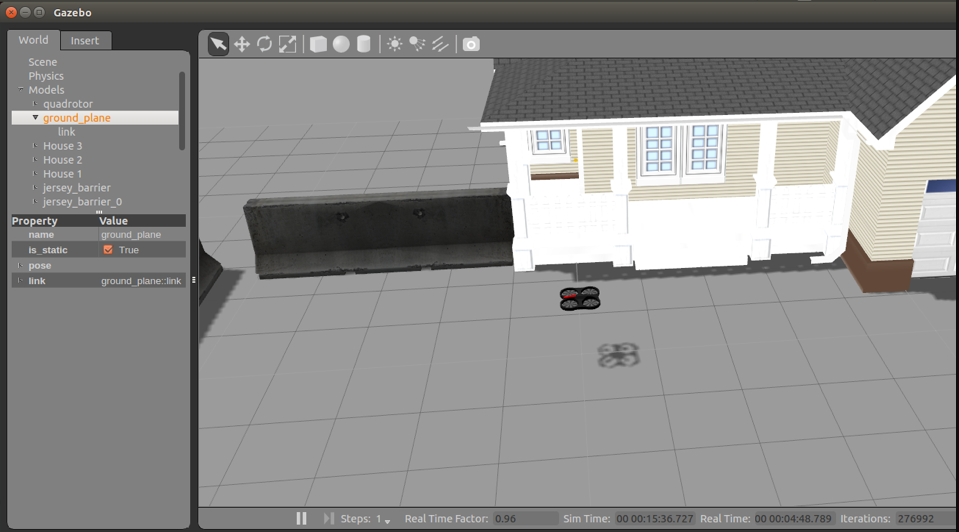
\includegraphics[scale=0.50]{img/gazebo.PNG}
  	\caption{Entorno de simulación Gazebo}
  	\label{fig:gazebo}
\end{figure}

\section{ROS}
\label{sec:ros}

Es un framework para el desarrollo de software para robots que provee la funcionalidad de un sistema operativo en un clúster heterogéneo. ROS (Robot Operating System) proporciona bibliotecas y herramientas para ayudar a los desarrolladores de software a crear aplicaciones de robots. Proporciona abstracción de hardware, controladores de dispositivo, bibliotecas, visualizadores, paso de mensajes, administración de paquetes y más.

 Es completamente de código abierto (BSD) y gratuito para que otros lo usen, cambien y comercialicen. SU objetivo principal es permitir que los desarrolladores de software creen aplicaciones de robots más capaces de forma rápida y fácil en una plataforma común.

ROS se desarrolló originalmente en 2007 bajo el nombre de switchyard por el Laboratorio de Inteligencia Artificial de Stanford.
 
Desde 2008, el desarrollo continua primordialmente en Willow Garage, un instituto de investigación robótico con más de veinte instituciones colaborando en un modelo de desarrollo federado

Vamos a describir a desde una perspectiva a muy alto nivel los conceptos básicos en los que se basa su arquitectura.


\subsection{Maestro ROS}
El Maestro permite que todas las demás piezas de software de ROS (Nodos) encuentren y hablen entre sí. Sin el Maestro, los nodos no podrían encontrarse, intercambiar mensajes o invocar servicios. De esta forma, no tenemos que especificar nunca específicamente "Enviar esta información del sensor a esa computadora en 127.0.0.1. Podemos simplemente decirle al Nodo 1 que envíe mensajes al Nodo 2.
El ROS Master proporciona registro y búsqueda de nombres para el resto del gráfico de computación.

BIBLIOGRAfIA

\subsection{Nodos}
Algunos robots llevan varias computadoras, cada una de las cuales controla un subconjunto de los sensores o actuadores del robot. Incluso dentro de una sola computadora, a menudo es una buena idea dividir el software del robot en pequeñas partes independientes que cooperan para lograr el objetivo general. Para esto existen los nodos de ros.
Los nodos son procesos que realizan cálculos. ROS está diseñado para ser modular en una escala de grano fino; un sistema de control de robot generalmente comprende muchos nodos.
Por ejemplo, un nodo controla un láser, un nodo controla los motores de las ruedas, un nodo proporciona una vista gráfica del sustema y así sucesivamente. Un nodo ROS se escribo con el uso de una biblioteca cliente ROS, como roscpp o rospy, más alante describiremos en detalle el proceso de desarrollo de uno un nodo ros.

\subsection{Servidor de Parámetros}
El servidor de parámetros permite que los datos se almacenen por clave en una ubicación central. Actualmente es parte del Master.

\subsection{Mensajes}
Los nodos se comunican entre sí al pasar mensajes. Un mensaje es simplemente una estructura de datos, que comprende campos tipados. Los tipos primitivos estándar (entero, punto flotante, booleano, etc.) son compatibles, al igual que las matrices de tipos primitivos. Los mensajes pueden incluir estructuras y matrices anidadas arbitrariamente (al igual que las estructuras C).

\begin{figure}[H]
    \centering
    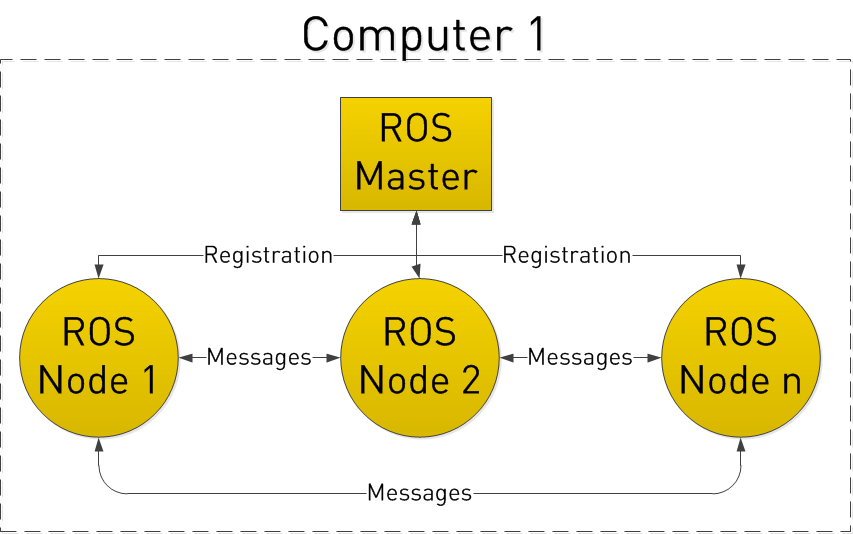
\includegraphics[scale=0.45]{img/ros-architecture.png}
  	\caption{Arquitectura básica ROS maestro-nodo}
  	\label{fig:ros-arch}
\end{figure}

\subsection{Topics o Temas}
Los mensajes se enrutan a través de un sistema de transporte con semántica de publicación suscripción. Un nodo envía un mensaje publicándolo en un tema determinado. El tema es un nombre que se usa para identificar el contenido del mensaje. Un nodo que está interesado en cierto tipo de datos se suscribirá al tema apropiado. Puede haber varios editores y suscriptores simultáneos para un único tema, y un solo nodo puede publicar y / o suscribirse a múltiples temas. En general, los editores y los suscriptores no conocen la existencia de los demás. La idea es desacoplar la producción de información de su consumo. Lógicamente, uno puede pensar en un tema como un bus de mensajes fuertemente tipado. Cada bus tiene un nombre, y cualquiera puede conectarse al bus para enviar o recibir mensajes, siempre que sean del tipo correcto.

\subsection{Servicios}
El modelo de publicación / suscripción es un paradigma de comunicación muy flexible, pero su transporte unidireccional de muchos a muchos no es apropiado para las interacciones de solicitud / respuesta, que a menudo se requieren en un sistema distribuido. La solicitud / respuesta se realiza a través de servicios, que están definidos por un par de estructuras de mensaje: una para la solicitud y otra para la respuesta. Un nodo proveedor ofrece un servicio con un nombre y un cliente usa el servicio enviando el mensaje de solicitud y esperando la respuesta. Las bibliotecas cliente de ROS generalmente presentan esta interacción al programador como si fuera una llamada de procedimiento remoto.

\begin{figure}[H]
    \centering
    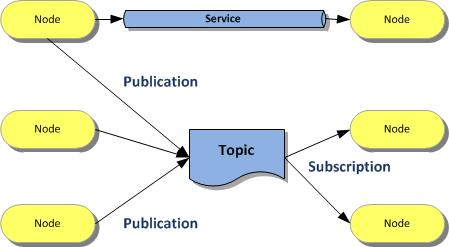
\includegraphics[scale=1]{img/ros-architecture-3.jpg}
  	\caption{Arquitectura básica ROS publicación-suscripción}
  	\label{fig:ros-servicio}
\end{figure}


\cleardoublepage
\chapter{Desarrollo}
Una vez presentado el contexto, los objetivos, así como las herramientas empleadas, en este capítulo se detalla la mejora desarrollada sobre la herramienta Scratch4Robots. Primero presentamos el diseño global y después analizaremos en detalle que aportaciones se han realizado y como se han llevado a cabo.
\section{Diseño}
\label{sec:diseno}
Como diseño general de la herramienta, y la forma más sencilla de apreciar la sencillez con la que el usuario tiene que lidiar sería el siguiente esquema:
\begin{figure}[H]
    \centering
    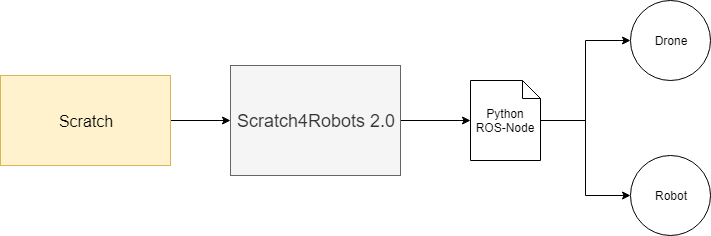
\includegraphics[scale=0.6]{img/s4r-diagram2.png}
  	\caption{Diseño de Scratch4Robots}
  	\label{fig:s4r}
\end{figure}

Para englobar todos los componentes ya definidos en un mismo contexto vamos a definir la arquitectura y diseño de la herramienta.
\begin{figure}[H]
    \centering
    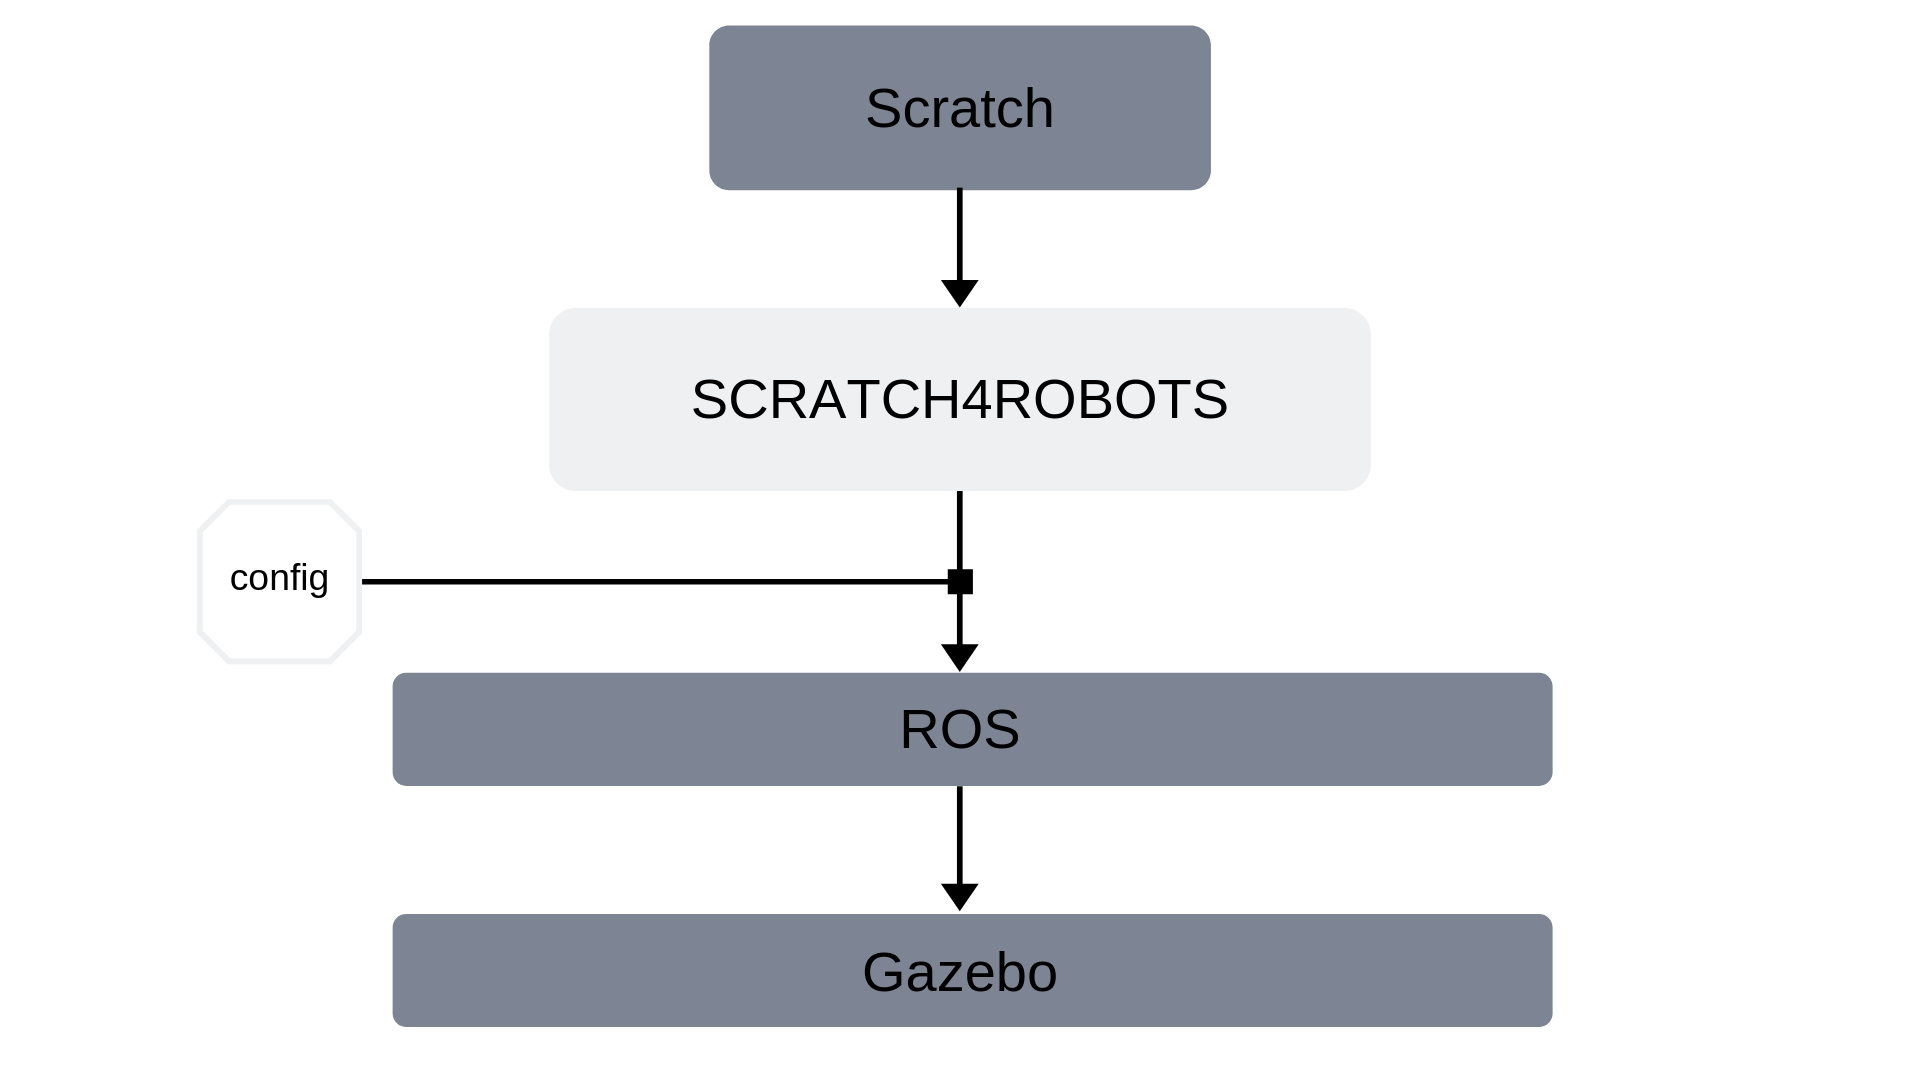
\includegraphics[scale=0.30]{img/diseno.jpg}
  	\caption{Diseño del contexto global de Scratch4Robots}
  	\label{fig:s4r}
\end{figure}
Partimos de un proyecto generado en el lenguaje de programación visual Scratch, al que se le ha agregado una serie de bloques robóticos, definidos e implementados por nosotros. Con estos nuevos bloques y los ya disponibles en Scratch se programará la lógica que queremos que siga nuestro robot.\\

Una vez tenemos nuestro proyecto, Scratch4Robots se encarga de la traducción de este proyecto a un nodo ROS, programado en Python, que con un único fichero de configuración en el que indicamos los tópicos que vamos a necesitar, se encuentra listo para su ejecución sobre un robot en un entorno simulado, por ejemplo Gazebo.\\

Esta traducción como hemos dicho devuelve un nodo ROS programado en Python, esto lo conseguimos introduciendo el código programado en scratch en una plantilla en la que se predefine toda la lógica necesaria para su ejecución.\\

Esta encapsulación del código generado en un nodo ROS la hemos conseguido través de la siguiente plantilla predefinida por nostros:

\begin{lstlisting}[language=python,firstnumber=1]
#!/usr/bin/env python
# -*- coding: utf-8 -*-n
import time
import config
import sys
import os
import yaml
import math
# Establece la subscripcion a topics ROS para drones
from drone import Drone 
# Establece la subscripcion a topics ROS para robots
from robot import Robot 

def execute(robot):
    try:
    # Desde codigo, insertamos la traduccion obtenida aqui 
    //
    except KeyboardInterrupt:
        raise
        
if __name__ == '__main__':
    if len(sys.argv) == 2:
        path = os.getcwd()
        open_path = path+'/'
        filename = sys.argv[1]
    else:
        sys.exit("ERROR: Example:python my_generated_script.py cfgfile.yml")
    # carga de configuraciones, topics ros a los que nos suscribimos, a traves de fichero yml.
    if os.path.isabs(filename):
        stream = open(filename, "r")
        cfg = config.load(filename)
    else:
        stream = open(open_path + filename, "r")
        cfg = config.load(open_path + filename)
        yml_file = yaml.load(stream)
        
    for section in yml_file:
    # En el yml de configuracion se define si se trata de robot o drone.
    if section == 'drone':
        # Si es drone se inicia la clase que hace la subscripcion a todos los topics ROS
        robot = Drone(cfg)
    	break
    elif section == 'robot':
    	# De forma analoga si se trata de un robot sobre ruedas
        robot = Robot(cfg)
    	break
    # Ejecutamos el codigo generado, ya con todas las subscriciones a ROS hechas
    execute(robot)

\end{lstlisting}


Esta plantilla abstrae de toda la dificultad tras la publicación y suscripción a tópicos ROS, y junto con el código traducido desde Scratch será el nodo final que el usuario ejecutará. Pero el proceso que hemos realizado para la completa integración con ROS no acaba aquí. Como se ve en la plantilla anterior, la suscripción a los topics se realiza a través de las librerías \textit{drone} y \textit{robot}. Esto se hace de cara a no sobrecargar el Nodo generado, con código que requiere de cierto nivel de entendimiento sobre la arquitectura ROS. Estos modulos python, que se facilita su uso mediante la instalación de los paquetes pip robot-scratch4robots y drone-scratch4robots, se encargan de la suscripción y publicación a los tópicos en los que nuestro robot simulado estrá conectado. Estas librerías han sido generados en su totalidad en esta versión de la herramienta, Scratch4Robots 2.0.\\

\begin{figure}[H]
    \centering
    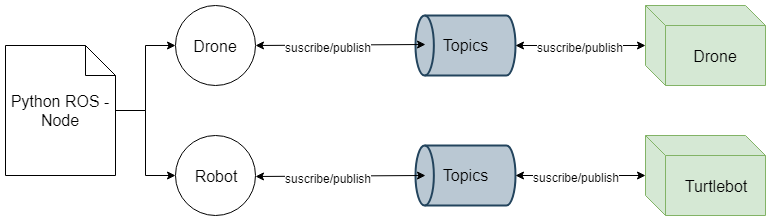
\includegraphics[scale=0.6]{img/s4r-diagrama-robot.png}
  	\caption{Esquema de funcionamiento del Nodo ROS en Python}
  	\label{fig:s4r-esquema}
\end{figure}

Entrando en más detalle de estas librerías, vamos a ver como realiza la suscripción y publicación en los tópicos desde una de ellas, con fragmentos de códigos obtenidos de la aplicación.\\

\begin{lstlisting}[language=python,firstnumber=1]
import config
import rospy

class Robot():
    def __init__(self, cfg):
        # inicia nodo ROS Robot
        self.__node = rospy.init_node("robot", anonymous=True)
        # hacemos la subscripcion a los topics ROS
        topic = cfg.getProperty("robot.Pose3D.Topic")
        self.__pose3d_client = ListenerPose3d(topic)
        topic = cfg.getProperty("robot.Motors.Topic")
        self.__motors_client =  PublisherMotors(topic)
\end{lstlisting}

Describiendo el fragmento de código anterior y como se aprecia en el esquema de más arriba, nuestro nodo ROS en Python, a través del objeto Python \textit{Robot}, hace la carga de propiedades del cfg que se le pasa como argumento. Estas propiedades como hemos comentado anteriormente serán los tópicos a los que se conectará nuestro nodo. Se realizará la suscripción a cada tópico de manera individual. En este caso y observando el código,  usamos el objeto \textit{ListenerPose3d}, para conectarnos al tópico de el que obtendremos la información publicada por el sensor de odometría del robot, del mismo modo se hace con \textit{PublisherMotors} para el uso de los motores del robot.\\

En el siguiente extracto de código se aprecia simplificado el detalle de una de las clases que realizan la suscripción, y de las obtenemos información del robot a través de mensajes ROS, publicados en un tópico.

\begin{lstlisting}[language=python,firstnumber=1]
# modulo python oficial ros
import rospy
# mensajes de comunicacion ROS para la lectura de odometria
from nav_msgs.msg import Odometry
class ListenerPose3d:
    def __init__(self, topic):
    	# Objeto Pose3d() contiene los datos devueltos por el sensor
        self.data = Pose3d() 
        # Al suscribirnos como argumento se introduce el topico,
        # el tipo de mensaje ROS que se lee del topico
# y una funcion de callback en la que recogemos las lecturas del topico
        self.sub = rospy.Subscriber(self.topic, Odometry, self.__callback)

    def __callback (self, odom):
        pose = odometry2Pose3D(odom)
        self.lock.acquire()
        self.data = pose
        self.lock.release()
        
    # metodo a traves del cual obtendremos la pose 3d    
    def getPose3d(self):
        self.lock.acquire()
        pose = self.data
        self.lock.release()
        return pose
\end{lstlisting}

Este mismo procedimiento hay que seguirlo para cada uno de los posibles tópicos ROS que necesite nuestra aplicación, por ejemplo, uno para dar velocidad a los distintos motores, otro para el sensor láser, cámaras incrustadas en el robot etcétera.

Con todo esto se puede apreciar la complejidad de la que evadimos al usuario, siendo para él, un simple ejecutable o nodo, completamente operativo, generado a través de nuestra aplicación. Una vez lanzado el nodo habremos sido capaces de aplicar una lógica programada en Scratch sobre un robot en un entorno simulado. 


\section{Desarrollo de bloques}
\label{sec:desarrollo-de-bloques}

Una de las aportaciones de este trabajo a la herramienta ha sido la refactorización de bloques ya existentes y la agregación de nuevos bloques funcionales.
En la programación visual entendemos por bloque a cada componente visual que contiene una lógica específica, con la agrupación de bloques podemos conseguir un flujo de programación complejo. En primer lugar vamos a describir como agregar estos nuevos bloques a Scratch, siguiendo con su definición e implementación.

\subsection{Extensión de Scratch}

Scratch facilita el uso de bloques personalizados mediante extensiones externas, estas  extensiones externas a la aplicación se definen mediante el uso de ficheros JSON, aunque por convención, en Scratch tendrán extensión .s2e. Este tipo de ficheros se creó para la comunicación mediante HTTP de bloques con aplicaciones auxiliares, por ejemplo algún tipo de hardware. Nosotros no vamos a utilizar esta funcionalidad, únicamente nos ayudamos de este documento .s2e para definir nuestra extensión y pueda ser usada desde el IDE offline de scratch.\\

En este documento se define un objeto JSON, el cual será la definición de la extensión, en el que se incluye el nombre de la extensión, un puerto usado para la comunicación de componentes externos en caso de ser necesario y una lista de bloques de Scratch. \\

A continuación se define un ejemplo de una extensión para Scratch. 
\begin{lstlisting}[language=json,firstnumber=1]
{ 
  "extensionName": "Extension Example",
  "extensionPort": 12345,
  "blockSpecs": [
    [" ", "beep", "playBeep"],
	[" ", "set beep volume to %n", "setVolume", 5],
	["r", "beep volume", "volume"],
  ]
}
\end{lstlisting}

El campo ``blockSpecs'' describe los bloques de extensión que aparecerán en el apartado ``Más bloques'' en la aplicación de Scratch.
En en este caso, hay tres bloques:
\begin{itemize}
\item Un bloque de comandos que reproduce un pitido.
\item Un bloque de comando que
establece el volumen del pitido.
\item Un bloque que devuelve un valor, que informa del volumen de un pitido.
\end{itemize}

Cada bloque se describe mediante una matriz con los siguientes campos:
\begin{itemize}
\item \textbf{Tipo de bloque}:

\begin{itemize}
\item ' ' - bloque de comandos
\item 'w' - bloque de comandos que esperan
\item 'r' - bloque que retorna un valor
\item 'b' - bloque que retorna un booleano 
\end{itemize}
\item \textbf{Formato de bloque}:

El formato de bloque es una cadena que describe las etiquetas y ranuras de parámetros que aparecen en el bloque.
Las ranuras de parámetros están indicadas por una palabra que comienza con '\%' y puede ser una de:
\begin{itemize}
\item \%n -  parámetro de número 
\item \%s - parámetro de cadena 
\item \%b - parámetro booleano
\end{itemize}
\item \textbf{Operación o nombre de variable remota}:

El campo de operación en una especificación de bloque se usa de dos maneras. Para bloques de comandos, se envía a la aplicación auxiliar, junto con cualquier valor de parámetro, para invocar una operación. O para retornar bloques, es el nombre de una variable de sensor. Los valores de la variable del sensor se guardan en un diccionario.
La ejecución de un bloque simplemente devuelve el valor reportado más recientemente para esa variable de sensor.
\item \textbf{Parámetros predeterminados}:

Se pueden añadir cero o más valores de parámetros predeterminados

\item \textbf{Menús desplegables}:

Los bloques que definimos pueden hacer uso de parámetros de menú, los cuales definiremos de dos formas:
\begin{itemize}
\item \%m.menuName - parámetro de menú (no editable), proporciona un sencillo espacio para los parámetros del menú desplegable.
\item \%d.menuName - parámetro de número editable con menú, proporciona una ranura de parámetro numérico con un menú auxiliar.
\end{itemize}
\end{itemize}

Con todo esto podemos entender la definición de alguno de nuestros bloques como podemos en el siguiente extracto de código, en el que se ve la definición de algunos de nuestros bloques.
\begin{nobreak} 
\begin{lstlisting}[language=json,firstnumber=1]
{
  "extensionName": "Scratch4Robots",
  "extensionPort": 12345, 
  "blockSpecs": [
    ["", "stop robot-drone", "stop"],         
    ["", "move robot %m.robotDirections speed %n", "robot/move/speed", "forward", 1],
    ["r", "color detection %m.color", "camera/all","red"],
    ["r", "frontal laser distance", "laser/frontal"],
  ],
  "menus": {
    "robotDirections": ["forward", "back"],         
    "color": ["red", "blue"]
  }
}

\end{lstlisting}
\end{nobreak} 

\subsection{Bloques genéricos}
Antes de comenzar con los bloques propios a nuestra extensión vamos a necesitar una serie de bloques genéricos que nos ayuden a realizar lógica básica de programación como pueden ser operadores matemáticos, operadores lógicos y sentencias básicas de programación. Scratch ya nos ofrece estos bloques por definición, por lo que no hará falta agregarlos a nuestra extensión específica, solamente nos encargaremos de su posterior traducción a código Python.\\

A continuación mostramos todos los bloques genéricos de los que podemos hacer uso desde la herramienta Scratch4Robots, ya que hemos implementado su traducción a Python.

\begin{itemize}
\item \textbf{Bloques de operadores matemáticos}:

Bloques fundamentales de cara a realizar una lógica posterior con los datos obtenidos desde los sensores de nuestros robots, estos bloques son una de las mejoras ofrecidas por este trabajo.
\begin{figure}[H]
    	\centering
    	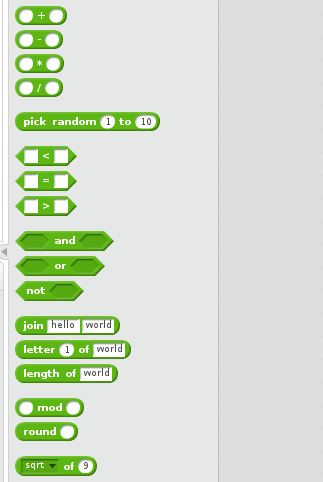
\includegraphics[scale=0.60]{img/bloques-mat.png}
     	\caption{Bloques matemáticos y lógicos}
  	\label{fig:mat}
\end{figure}

	\begin{itemize}

    \item \textbf{sqrt of ()}: Realiza la operación raíz cuadrada de un número dado
    \item \textbf{sin of ()}: Realiza la operación seno de un número dado
    \item \textbf{cos of ()}: Realiza la operación coseno de un número dado
    \item \textbf{tan of ()}: Realiza la operación tangente de un número dado
    \item \textbf{asin of ()}: Realiza la operación arcoseno de un número dado
    \item \textbf{acos of ()}: Realiza la operación arcocoseno de un número dado
    \item \textbf{atan of()}: Realiza la operación arcotangente de un número dado
    \item \textbf{log of ()}: Realiza la operación logaritmo de un número dado
    \item \textbf{ln of ()}: Realiza la operación logaritmo neperiano de un número dado
    \item \textbf{abs of ()}: Devuelve el valor absoluto de un número
    \item \textbf{mod of ()}: Devuelve el módulo de un número dado
    \end{itemize}

\item \textbf{Bloques de operadores lógicos}:
Permiten construir expresiones lógicas, se obtiene como resultado booleanos.
\begin{itemize}

 \item \textbf{And}: Operador de conjunción.
 \item \textbf{Or}: Operador de disyunción.
 \item \textbf{NOT}: Operador de negación.
 \item \textbf{Mayor que y Menor que}: Operadores de comparación numérica.
\end{itemize}

\item \textbf{Bloques de control}:

Estructuras de control básicas de programación.

\begin{figure}[H]
    	\centering
    	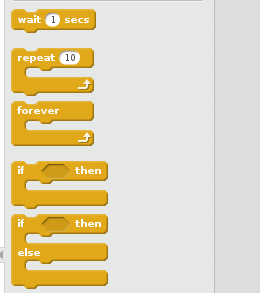
\includegraphics[scale=0.60]{img/bloques-control.png}
     	\caption{Bloques de control}
  	\label{fig:control}
\end{figure}
\begin{itemize}
\item \textbf{Wait () secs}: Pausa la ejecución el tiempo especificado, equivalente a la sentencia \textit{time.sleep()} de Python.
\item \textbf{Forever}: Bucle infinito, equivalente a \textit{while(True)} en lenguaje Python.
\item \textbf{If () then}: Comprueba la condición para que si la condición es verdadera, los bloques dentro de ella se ejecuten.
\item \textbf{If () Then, Else}: Comprueba la condición para que si la condición es verdadera, los bloques dentro de la primera condición se activen y si la condición es falsa, los bloques dentro de la segunda condición se activarán.
\item \textbf{Repeat ()}: Un ciclo que repite la cantidad de veces especificada, sería la equivalencia al bucle \textit{for} en Python.
\end{itemize}
\item \textbf{Otros}
\begin{itemize}

\item \textbf{say ()}: Imprime lo que le añadas como argumento, equivalente a \textit{print}.
\item \textbf{Set () to ()}: Utilizado para dar valor a una variable en concreto.
\end{itemize}

\item \textbf{Bloques de listas}:

Esta serie de bloques desarrollados en esta versión han sido de gran ayuda a la hora de la refactorización y creación de otros bloques de mayor complejidad.

\begin{figure}[H]
     	\centering
     	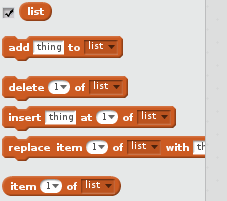
\includegraphics[scale=0.60]{img/bloques-listas.png}
     	\caption{Bloques de listas}
  	\label{fig:listas}
\end{figure}

\begin{itemize}
\item \textbf{Insert () at () of ()}: Inserta elemento en la posición seleccionada de la lista indicada.
\item \textbf{Item () of ()}: Devuelve el elemento almacenado en la posición indicada de la lista.
\item \textbf{Add () to ()}: Inserta en la lista un elemento.
\item \textbf{Delete () of ()}: Elimina el elemento en una posición determinada de la lista.
\end{itemize}
\end{itemize}

\subsection{Bloques para drones}
Estos bloques ya pertenecen a la extensión creada para la herramienta.
En este trabajo se ha realizado una refactorización completa de todos los bloques referentes a drones y la agregación de nuevos bloques. 

Cabe destacar de estos bloques que una vez traducidos al nodo final, que se consigue implementar el funcionamiento de drones bajo comunicación ROS, ésto es algo elaborado completamente en este trabajo.\\

Para ello nos apoyamos en MAVROS\footnote{\url{http://wiki.ros.org/mavros}}, puente oficial entre nodos ROS y Mavlink\footnote{\url{https://github.com/mavlink}}, el protocolo de comunicación estándar para drones.

\begin{itemize}
\item \textbf{Bloques perceptivos}:
Nos permiten obtener información de sensores incorporados en el drone.
	\begin{itemize}
	\item \textbf{Get pose3D}: Obtiene el valor de la posición 3D del robot.
		\begin{figure}[H]
     		\centering
     		
\includegraphics[scale=1.2]{img/block-pose.png}
     		\caption{bloque que retorna la posición del robot}
  		\label{fig:listas}
		\end{figure}
Simplificando la totalidad del código, la función Python en la que quedaría traducida sería \textit{getPose3d}, como se muestra:\\

\begin{lstlisting}[language=python,firstnumber=1]
class Drone():
    def __init__:
        client__pose3d = suscribePose3d(topic)
    def getPose3d(self):
        return client__pose3d.getPose3d
\end{lstlisting}
	\item \textbf{Color detection}: Nuevo componente añadido en esta versión, que haciendo uso de una cámara en el robot, detecta objetos de un determinado color, introducido como argumento, devolviendo una lista que contendrá las posiciones en los ejes x e y, además del tamaño del objeto, en la imagen capturada por la cámara.\\
	\begin{figure}[H]
     		\centering
     		
\includegraphics[scale=1.2]{img/block-color.png}
     		\caption{bloque que detecta objetos de un determinado color}
  		\label{fig:listas}
  				\end{figure}
  				
 Usando la biblioteca OpenCV de Python y con técnicas de análisis computacional de imágenes, de una simple imagen somos capaces de obtener su posición en la imagen y su tamaño:\\
 
 \begin{lstlisting}[language=python,firstnumber=1]
    def detect_object(self, color):
        # define the lower and upper boundaries of the basic colors
        color_range = __get_color_range(color)
        # get image type from camera ROS client
        image = self.__camera_client.getImage()
        # apply color filters to the image
        filtered_image = cv2.inRange(image.data, color_range[0], color_range[1])
        rgb = cv2.cvtColor(image.data, cv2.COLOR_BGR2RGB)
        # Apply threshold to the masked image
        ret,thresh = cv2.threshold(filtered_image,127,255,0)
        im,contours,hierarchy = cv2.findContours(thresh,cv2.RETR_TREE,cv2.CHAIN_APPROX_SIMPLE)
        # Find the index of the largest contour
        for c in contours:
            if c.any != 0:
                areas = [cv2.contourArea(c) for c in contours]
                max_index = np.argmax(areas)
                cnt=contours[max_index]
                if max(areas) > 0.0:
                    x,y,w,h = cv2.boundingRect(cnt)
                    x_position = (w/2)+x
                    y_position = (h/2)+y
                    size = w*h
        return size, x_position, y_position
\end{lstlisting}


	\end{itemize}
\item \textbf{Bloques de movimiento}
	\begin{itemize}
	\item \textbf{Stop robot-drone}: Pone a su valor inicial todas las velocidades del robot.\\
	\begin{figure}[H]
     		\centering
     		
\includegraphics[scale=1.2]{img/block-stop.png}
     		\caption{bloque stop-robot}
  		\label{fig:listas}
  				\end{figure}
Con el código que se ejecutará tras su traducción:\\

 \begin{lstlisting}[language=python,firstnumber=1]
    def stop_robot(self):
        self.client__vel.sendVelocities(0,0,0,0,0,0)
        time.sleep(1)

\end{lstlisting}

	\item \textbf{Drone take off}: Hace que el drone despegue.\\
	\begin{figure}[H]
     		\centering
     		
\includegraphics[scale=1.2]{img/block-takeoff.png}
     		\caption{bloque que realiza el despegue del drone}
  		\label{fig:listas}
  				\end{figure}
  				
Mediante el armado del drone y el envío de una velocidad ascendente conseguimos su despegue:\\

 \begin{lstlisting}[language=python,firstnumber=1]
    def takeoff(self):
        self.client__extra.arming()
        self.client__vel.sendVelocities(0,0,2,0,0,0)
        time.sleep(1)
        self.client__vel.sendVelocities(0,0,0,0,0,0)
\end{lstlisting}

	\item \textbf{Drone land}: Realiza un aterrizaje controlado del drone.\\
	\begin{figure}[H]
     		\centering
     		
\includegraphics[scale=1.2]{img/block-land.png}
     		\caption{bloque que realiza el aterrizaje del drone}
  		\label{fig:listas}
  				\end{figure}
Para realizar el aterrizaje del drone a través de ROS, tiene su propio tópico al cual se le envía una llamada con argumentos cero, como se puede observar:\\

 \begin{lstlisting}[language=python,firstnumber=1]
    def land(self):
        self.lock.acquire()
        self.land_client.call(0,0,0,0,0)
        self.lock.release()
\end{lstlisting}
	

	\item \textbf{Move drone}: Bloque que tras la refactorización admite una lista con las velocidades del drone en los diferentes ejes (velocidad en el eje x, velocidad en el eje z, velocidad yaw), pare realizar giros se debe combinar la velocidad en el eje x con la velocidad de rotación en yaw.\\
	\begin{figure}[H]
     		\centering
     		
\includegraphics[scale=1.2]{img/block-move-drone.png}
     		\caption{bloque que realiza el despegue del drone}
  		\label{fig:listas}
  	\end{figure}
  	
Lo que se traduce a python con la siguiente función:\\
  	
\begin{lstlisting}[language=python,firstnumber=1]
 def move_vector(self, velocities):
    # cliente que realiza la suscripcion al topico que envia velocidades
    pose = self.client__pose3d.getPose3d()
    yaw = pose.yaw
    vx = velocities[0]
    vz = velocities[1]
    az = velocities[2]
    vxt = vx*math.cos(yaw)
    # cliente que realiza la suscripcion al topico que envia velocidades
    self.client__vel.sendVelocities(vxt,0,vz,0,0,az)
\end{lstlisting}
	
	Para clarificar la creación del cliente, y ver donde se realiza la comunicación ROS realmente se adjunta un estracto de código en el que se simplifica el cliente que publica el tópico en el que se van a enviar las velocidades al drone.\\
	
\begin{lstlisting}[language=python,firstnumber=1]
class publisher_motors:
    # simplificando el codigo del cliente
    def __init__(self, topic):
        self.pub = rospy.Publisher(topic, TwistStamped, queue_size=1)

    def sendVelocities(vx,vy,vz,ax,ay,az):
        tw = vel2twisted(vx,vy,vz,ax,ay,az)
        self.pub.publish(tw)
\end{lstlisting}
	
	\end{itemize}
\end{itemize}



\subsection{Bloques para robots con ruedas}
\begin{itemize}
\item \textbf{Bloques perceptivos}
	\begin{itemize}
	\item \textbf{Pose3D} :Obtiene el valor de la posición 3D del robot.
		\begin{figure}[H]
     		\centering
     		
\includegraphics[scale=1.2]{img/block-pose.png}
     		\caption{bloque pose del robot}
  		\label{fig:listas}
  	\end{figure}
Se traduce de forma equivalente a su homólogo para drones, la única diferencia es el tópico desde el que recibe la información.\\
 
	\item \textbf{Color detection}: Bloque homólogo al del drone, dado un color nos devuelve su posición en la imagen, y su tamaño.
		\begin{figure}[H]
     		\centering
     		
\includegraphics[scale=1.2]{img/block-color.png}
     		\caption{bloque que detecta colores en una imagen}
  		\label{fig:listas}
  	\end{figure}
Se trata del mismo bloque perceptivo ya definido para drones.\\

\item \textbf{Frontal distance}: Obtiene la medida promedio de los datos del láser frontal. 
		\begin{figure}[H]
     		\centering
     		
\includegraphics[scale=1.2]{img/block-laser.png}
     		\caption{bloque que devuelve datos de un laser}
  		\label{fig:listas}
  	\end{figure}
Se traduce al siguiente método Python:\\

\begin{lstlisting}[language=python,firstnumber=1]
def get_laser_distance(self):
        # get laser values from ROS client
        laser = self.__laser_client.getLaserData()
        l = [x for x in laser.values if str(x) != 'nan' and x < 10]
        try:
            avg = sum(l) / len(l)
        except ZeroDivisionError:
            avg = 0
        return avg
\end{lstlisting}

	\end{itemize}
\item \textbf{Bloques de movimiento}
	\begin{itemize}

	\item \textbf{robot move ()}: Admite como parámetro una lista con las velocidades en el eje x e y.
		\begin{figure}[H]
     		\centering
     		
\includegraphics[scale=1.2]{img/block-move-robot.png}
     		\caption{bloque de movimiento para robots}
  		\label{fig:listas}
  	\end{figure}
  	
Con su traducción:\\

\begin{lstlisting}[language=python,firstnumber=1]
    def move_vector(self, velocities):
        vx = float(velocities[0])
        vz = float(velocities[1])
        print "velocities:",vx,vz
        self.__reset()
        self.__vel.vx = vx
        self.__vel.vz = vz
        if vz>0:
            self.turn("left",vz)
        if vz<0:
            self.turn("right",vz)
        self.__publish(self.__vel)
\end{lstlisting}

	\item \textbf{robot turn ()}: Permite la rotación sobre el propio eje del robot.
	\begin{figure}[H]
     		\centering
     		
\includegraphics[scale=1.2]{img/block-turn.png}
     		\caption{bloque que realiza el giro del robot}
  		\label{fig:listas}
  	\end{figure}
  	
Con su traducción Python:\\

\begin{lstlisting}[language=python,firstnumber=1]
    def turn(self, direction, vel):
        self.__vel.az = vel
        # set different direction
        if direction == "right":
            self.__vel.az = -self.__vel.az
        # publish movement
        self.__publish(self.__vel)
\end{lstlisting}
	\end{itemize}
\end{itemize}

Con esto se definen los bloques pertenecientes a nuestra extensión, de la forma en que Scratch los muestra y la traducción de cada uno de ellos llevada, de una forma simplificada. Se aprecia que se trata de robots sofisticados, con cierta complejidad. La cual hacemos transparente para el usuario, simplificando toda la lógica que existe tras cada robot, en simples e intuitivos bloques gráficos.

\section{Traducción de bloques}
El último paso será definir la estrategia que vamos a seguir para realizar la traducción de los bloques creados anteriormente, al nodo ROS final, programado en Python.

Vamos a estudiar más a fondo como trabaja la biblioteca Kurt y cómo nos ha ayudado en la traducción de bloques.\\

Kurt es una biblioteca de Python que permite la manipulación compleja de proyectos Scratch (archivos .sb o .sb2) a través de simples comandos de Python. Incluye un decompilador, que permite que un proyecto se cargue en un conjunto de objetos de Python, y un compilador que permite el empaquetamiento de un conjunto de scripts de imágenes / texto en proyectos scratch.\\

En este proyecto se ha utilizado una versión\footnote{\url{https://pypi.org/project/jderobot-kurt/}} mejorada de esta biblioteca, con ciertas adaptaciones para el tratamiento de extensiones externas como la nuestra. Kurt define los bloques usados por Scratch como objetos JSON, en esta nueva versión se agrega un fichero con la configuración de nuestros bloques como objetos JSON. De esta forma se agrega la capacidad de obtener la información de los bloques de nuestra extensión.\\

La clase principal de kurt almacena el contenido de un archivo de proyecto Scratch.
Los contenidos incluyen variables globales y listas, el escenario y los sprites, cada uno con sus propios scripts, sonidos, variables y listas.\\

Una vez obtenido el contenido de un proyecto Scratch en un objeto Python, con el siguiente fragmento de código somos capaces de obtener el String representativo de cada bloque.\\

\begin{lstlisting}[language=python,firstnumber=1]
# load the scratch project
p = kurt.Project.load(open_path + sys.argv[1])

# show the blocks included
for scriptable in p.sprites + [p.stage]:
	for script in scriptable.scripts:
		# exclude definition scripts
		if "define" not in script.blocks[0].stringify():
			s = script
print("Stringify:")
sentences = []
for b in s.blocks:
	print(b.stringify())
\end{lstlisting}

Una vez tenemos la lista de los Strings equivalentes a los bloques del proyecto Scratch, hay que realizar una tarea de transformación de estas a código Python.\\

En este trabajo se modifica de forma notable la forma en la que se realizaba de forma inicial esta traducción, agregando una gran cantidad de bloques soportados y añadiendo un grado de recursividad que permite la traducción de bloques anidados.\\

En la traducción nos apoyamos de unos diccionarios Python en los que mapeamos el string equivalente al bloque Scratch con el equivalente Python que queremos sustituir, esto nos lleva al último punto de nuestro desarrollo. Para ciertos bloques de Scratch existe una traducción directa a un comando Python como ya hemos visto antes. Mientras que para los bloques robóticos definidos por nuestra extensión debemos de crear un método específico que contenga toda la lógica a implementar como hemos visto anteriormente en la descripción de nuestros bloques.\\

En este trabajo hemos refactorizado la totalidad de la lógica tras los bloques robóticos, dándole una mayor coherencia a todos ellos. Además de crear lógica completamente nueva para ciertos bloques agregados en esta versión. Cabe destacar el bloque referente a la detección de objetos de un cierto color.\\

Además de la traducción, Scratch4Robots encapsula este código Python en un nodo ROS, que contiene todo lo necesario para su posterior ejecución, con el único requisito de un fichero de configuración en el que especificaremos los tópicos que va a necesitar nuestro nodo. Cerrando de esta forma el ciclo de trabajo de la herramienta.\\







\cleardoublepage
\chapter{Integración}
Una vez explicado los nuevos desarrollos efectuados para esta versión de la herramienta, vamos a centrarnos en uno de los puntos claves de este trabajo, la paquetización de Scratch4Robots 2.0, llegando a conseguir una fácil instalación e integración de esta. Esto lo conseguimos con un análisis de sus dependencias, desacoplando todas estas dependencias lo más que podamos para darle una mayor flexibilidad, y una vez desacopladas permitir la instalación de la herramienta, junto con sus dependencias de una forma sencilla, rápida y homogénea.

\section{Análisis de dependencias}
\label{sec:dependencias}
Partimos de una versión fuertemente acoplada con JdeRobot, siendo necesaria la instalación de toda la suite para el correcto funcionamiento de la herramienta. Esto añade una complejidad de instalación innecesaria a nuestra aplicación, cosa que no queremos ya que buscamos un uso educativo de ella, por lo que buscamos la mayor facilidad de instalación posible.\\

Como principal dependencia nos encontramos la biblioteca \textit{comm} de JdeRobot, biblioteca que como ya hemos explicado antes, abstrae al programador del tipo de comunicación que se quiera establecer con el robot final, pudiendo con un mismo punto de entrada, entablar una comunicación vía ROS o vía ICE. En este trabajo nos hemos centrado en la comunicación mediante ROS, por lo que se ha realizado una tarea de desacople de las funcionalidades ROS de la biblioteca \textit{comm}. El resultado de esta tarea de desacople es la creación de una nueva biblioteca, basada puramente en comunicación ROS.\\

Esta biblioteca llamada \textit{commros}S será la encargada de crear y gestionar las comunicaciones entre nodos ROS de nuestras aplicaciones. Desde la publicación y suscripción de nodos, hasta el envío de mensajes a través de ellos.\\

A su vez, la propia biblioteca \textit{comm} tenía dependencias con otras librería del entorno JdeRobot, en algunos casos hemos optado por refactorizar las clases puramente ROS, ya desacopladas de \textit{comm}, para que no hagan uso de estas dependencias. Mientras que en algunos casos, viendo la utilidad de estas librerías, se han optado por incorporar a nuestro proyecto. Un ejemplo de esta reutilización es la biblioteca \textit{Config} de JdeRobot.\\

Para comprender la importancia de esta dependencia vamos a explicar brevemente su funcionalidad. Esta biblioteca ayuda a la carga de propiedades mediante un fichero .yml, que mediante una simple API, busca y retorna cualquier propiedad que se haya definido en este fichero. En nuestro caso es extremadamente útil, ya que podemos adaptar nuestro nodo ROS a cualquier robot y situación. Como hemos explicado anteriormente, ROS establece comunicación a través de nodos mediante la publicación de tópicos, a los que el resto de nodos podrán subscribirse. En este fichero de comunicación establecemos los tópicos de los que se va a nutrir nuestro nodo, mediante la librería \textit{Config} carga estos nodos y con las utilidades de la biblioteca ya mencionada \textit{commros}, se suscribie y publica en esos tópicos.\\

Éstas serían las dependencias con respecto a JdeRobot, pero nuestra herramienta contiene dependencias externas. La más importante es con la ya conocida biblioteca Kurt, parte esencial en nuestro trabajo de traducción, y por lo tanto en el funcionamiento de la herramienta. Otra dependencia de importancia en nuestro proyecto es con la biblioteca OpenCV, la cual nos permite el análisis computacional de imágenes, y por lo tanto que nuestro bloque de visión funcione correctamente.

\section{Creación y publicación de paquetes pip}
\label{sec:pip}
Una vez hecho el análisis y desacoplo en mayor medida de nuestro código con estas dependencias, buscamos la forma de facilitar la instalación de nuestra herramienta.\\

Con todo esto hemos dejado el camino preparado para conseguir que nuestra herramienta no sea un programa monolítico, en el que se encuentran incrustadas todas sus librerías y funcionalidades, teniendo que actualizar toda herramienta cada vez que ésta sufra un mínimo cambio en cualquiera de sus dependencias. \\

Para dar el paso de una aplicación monolítica a una distribuida, lo conseguimos mediante la paquetización de estas dependencias en paquetes pip\footnote{\url{https://pip.pypa.io/en/stable/}} independientes.\\

Pip es un sistema de administración de paquetes utilizado para instalar y administrar paquetes de software escritos en Python. Todos los paquetes pip pueden encontrarse en el Python Package Index (PyPi)\footnote{\url{https://pypi.org/}}, siendo accesibles para todo el mundo en cualquier momento. Es fácil ver el potencial de este sistema, subiendo nuestras dependencias a PyPi somos capaces de instalar todas ellas de una sola atacada.\\

Para crear estos paquetes pip se genera en un directorio una estructura de ficheros específica, entre las que se encontrarán por su puesto nuestro módulo y un archivo llamado \textit{setup.py}. Aquí se configura todo nuestro paquete, desde su nombre, versión, dirección del código fuente o incluso dependencias que necesite y se instalarán a su vez de forma automática.\\

El siguiente paso es generar \textit{paquetes de distribución} para el paquete. Estos son los archivos que se cargan en el índice de paquetes (PyPi) y pueden ser instalados por pip por el usuario final.\\

Para este trabajo se han generado los siguientes paquetes pip para cada una de las dependencias que tenía nuestra herramienta:

\begin{itemize}
\item \textbf{jderobot-ros}\footnote{\url{https://pypi.org/project/jderobot-ros/}}:

Contiene todo lo referente a la publicación y suscripción de Tópicos ROS. 
\item \textbf{config-jderobot}\footnote{\url{https://pypi.org/project/config-jderobot/}}:

Ayuda a la carga de propiedades desde un fichero de configuración, estas propiedades en nuestro caso serán los Topicos que necesita nuestro nodo para funcionar. 
\item \textbf{jderobot-jderobottypes}\footnote{\url{https://pypi.org/project/jderobot-jderobottypes/}}:

Abstracción de tipos de datos, simplificándolos para un más fácil uso de ellos.
\item \textbf{jderobot-kurt}\footnote{\url{https://pypi.org/project/jderobot-kurt/}}:

Contiene la versión adaptada de la biblioteca para nuestro proyecto, haciendo posible la obtención de información de los bloques definidos en la extensión Scratch que hemos creado para nuestra herramienta.
\item \textbf{robot-scratch4robots}\footnote{\url{https://pypi.org/project/robot-scratch4robots/}}:

Modulo que contiene toda la lógica tras los bloques específicos de robots sobre ruedas que hemos creado para esta herramienta.
\item \textbf{drone-scratch4robots}\footnote{\url{https://pypi.org/project/drone-scratch4robots/}}:

Modulo que contiene toda la lógica tras los bloques específicos de drones que hemos creado para esta herramienta.
\end{itemize}


La publicación de estos paquete pip hace que sea instalable como cualquier otro módulo Python a través de linea de comandos:\\ 

\begin{lstlisting}[language=json,firstnumber=1]
~$ sudo pip install robot-scratch4robots drone-scratch4robots jderobot-kurt jderobot-jderobottypes jderobot-ros jderobot-config
\end{lstlisting}

Una vez instalado podremos hacer uso de ellos desde cualquier proyecto en nuestra máquina, como es el caso de nuestro propio paquete ROS, y los nodos generados tras su traducción.\\

Con esto hemos modularizado al máximo nuestra herramienta, consiguiendo poder mejorar y ampliar su funcionalidad sin necesidad de generar una nueva versión completa de nuestra herramienta, además de conseguir la instalación de todas nuestras dependencias con una facilidad asombrosa.
\section{Creación y publicación de paquete ROS}
\label{sec:paquete-ros}
Hasta ahora hemos externalizado nuestros módulos Python en paquetes pip, pero aún no hemos resuelto cómo facilitar el uso e instalación de nuestra herramienta, que como hemos expuesto, se trata de un nodo ROS. Antes de comenzar este trabajo la herramienta se basaba en un repositorio con el código fuente, el cual había que descargar al completo y manualmente instalar todo el entorno necesario para su correcto funcionamiento. Esto llegaba a ser engorroso e incluso complicado, ya que eran necesarias una gran cantidad de herramientas complementarias.\\

Una solución aportada en este trabajo es la creación de un paquete ROS y su posterior publicación a los repositorios públicos. Con esto, al igual que hemos hecho con los paquetes pip conseguimos que nuestra herramienta sea instalable como cualquier otro programa en un sistema operativo Ubuntu, mediante un solo comando. \\

Para la creación del paquete nos ayudamos de \textit{catkin}\footnote{\url{http://wiki.ros.org/catkin/conceptual_overview}}. Es el sistema de compilación oficial de ROS. Combina macros de CMake y scripts de Python para proporcionar alguna funcionalidad además del flujo de trabajo normal de CMake. El flujo de trabajo de \textit{catkin} es muy similar al de CMake, pero agrega soporte para la infraestructura automática de 'encontrar paquetes ROS' y al mismo tiempo construir múltiples proyectos dependientes. Esto se consigue gracias al sistema de compilación personalizada que usa \textit{catkin}.\\

Tras generar los ficheros de configuración necesarios de forma correcta, en los que indicamos las dependencias de la herramienta, los nodos que queremos exponer una vez esté instalado el paquete, e información referente a la distribución de ROS para la cual ha sido creado, nuestro paquete estará listo para ser generado.\\

En nuestro caso el nodo principal que queremos exponer, es el encargado de la traducción de Scratch a Python y genera el nodo final preparado par ser ejecutado sobre robots. Este nodo podrá ser ejecutado desde linea de comandos sin necesidad de disponer del código fuente de la aplicación, ya que estará instalado.\\

Para el último paso de nuestro proceso, la publicación del paquete, nos apoyamos de la herramienta \textit{bloom}\footnote{\url{http://wiki.ros.org/bloom}} proporcionada por la Open Source Robotics Foundation, que si hemos configurado correctamente nuestro paquete, automatizará la generación de los binarios que serán descargado por los usuarios finales, como se hace con cualquier otra instalación en Ubuntu. Tras realizar una petición al equipo que gestiona ROS y cumplir con los requisitos de calidad que ellos establecen, nuestro paquete será publicado.\\ 

La publicación del paquete hace que sea instalable en forma de binario, con el simple comando:\\ 

\begin{lstlisting}[language=json,firstnumber=1]
~$ sudo apt-get install ros-kinetic-scratch4robots
\end{lstlisting}

Una vez instalado podremos ejecutarlo desde linea de comandos con las facilidades que nos aporta ROS para el manejo de sus paquetes.\\

De esta forma hemos conseguido que Scratch4Robots\footnote{\url{http://wiki.ros.org/scratch4robots}} esté publicado de forma oficial como un paquete ROS, para su distribución Kinetic\footnote{\url{http://wiki.ros.org/kinetic}}, en repositorios públicos, además de todas sus dependencias. 


\section{Documentación de la herramienta}
\label{sec:documentación}
Por último, pero no por ello menos importante, cabe destacar la labor de documentación que se ha llevado a cabo en este trabajo. Una de las partes más importantes para el futuro uso de esta herramienta. La simpleza de uso, ayudada de una documentación clara, concisa y con ejemplos disponibles, hacen de nuestra aplicación idónea para aquellas personas con menos conocimientos técnicos.\\

En el repositorio oficial de Scratch4Robots\footnote{\url{https://github.com/JdeRobot/Scratch4Robots}} se indica paso a paso como realizar instalación y un primer ejemplo de uso, apoyado todo vídeos explicativos.\\

Además de los pasos para su instalación, se suministra un ejemplo para cada tipo de robot, robots con ruedas, y drones. Estos ejemplos contienen todo lo necesario para su ejecución en minutos, desde los proyectos Scratch ya generados, los ficheros de configuración necesarios para su ejecución, así como los comandos necesarios para la ejecución de los entornos simulados y una descripción detallada de su uso.\\

En la página oficial de JdeRobot, Scratch4Robots\footnote{\url{http://jderobot.org/Scratch4Robots}} se documenta en más detalle, en la que además de la guía de instalación y uso de la herramienta, se muestran todos los bloques disponibles, su forma de uso e incluso como puedes desarrollar tus propios bloques.\\

Con esto finalizamos la fase de integración de la herramienta, consiguiendo un entorno modular, de fácil instalación, y con guías de uso preparadas para usuarios con poco nivel técnico. Idóneo para niños y adultos con ganas de aprender a programar robots de forma sencilla y sin necesidad de gastar un tiempo desorbitado en el entendimiento en profundidad de éstos.



\cleardoublepage
\chapter{Experimentos}
En esta sección vamos a demostrar el potencial de la herramienta con algunos ejemplos de su funcionamiento. Validando el funcionamiento de ésta, y sus mejoras funcionales con respecto a la versión de Scratch4Robots de la que partimos.\\

Además de los ejemplos mostrados en este apartado, se ha creado una batería de pruebas con las que ver un ejemplo de funcionamiento de cada uno de nuestros bloques. Estas pruebas son proyectos Scratch, que el usuario puede cargar en el entorno de Scratch y usar como punto de partida para sus próximos proyectos.

\section{Evitar obstáculos con Turtlebot}
\label{sec:evitar-obstaculos}

En este ejemplo hacemos uso de un robot con ruedas, para ser más exactos de un Turtlebot. Para ejecutar las pruebas utilizamos Gazebo como simulador, cargando un entorno con obstáculos repartidos como se aprecia en la figura.\\

El objetivo directo de este experimento es la programación de un robot Turtlebot, capaz de evitar obstáculos de forma autónoma, con la ayuda de un sensor láser incorporado en su parte frontal. Esto lo vamos a conseguir usando únicamente la lógica de la que disponemos en Scratch junto con la extensión que aporta nuestra aplicación Scratch4Robots.\\
\pagebreak

Se puede apreciar con estos ejemplos el poder didáctico de la herramienta. Su simpleza y sencillez hacen de ella perfecta para la enseñanza a personas con pocos conocimientos técnicos.\\

Además este ejemplo podemos verlo en nuestro día a día con las famosas aspiradoras autónomas (iRobot Roomba), por lo que vemos una aplicación directa que podría tener nuestra aplicación fuera del ámbito didáctico.\\

Vamos a seguir el ciclo de vida de nuestra aplicación, explicando el proceso que lleva a la consecución de nuestro objetivo.\\

En primer lugar y con ayuda de nuestros bloques, desarrollamos la aplicación en Scratch. Una vez tenemos nuestro proyecto acabado y guardado, con la herramienta Scratch4Robots, ya instalada en nuestro equipo y mediante el uso de un solo comando realizaremos la traducción del proyecto.\\

\begin{figure}[H]
    \centering
    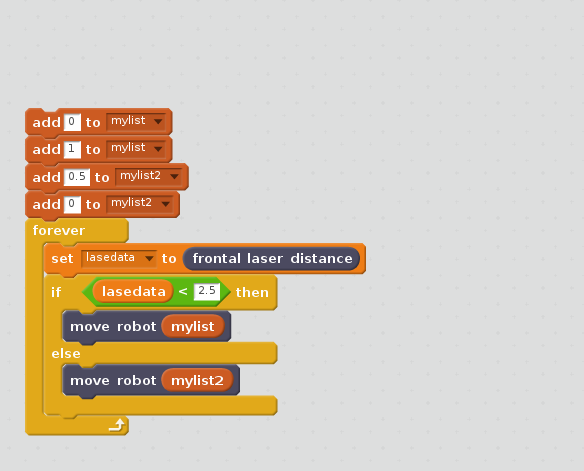
\includegraphics[scale=0.60]{img/robot-obstaculos-scratch.PNG}
  	\caption{Programación en Scratch del Turtlebot}
  	\label{fig:turtlebot}
\end{figure}
\pagebreak
Esta simpleza en la ejecución la conseguimos mediante las funcionalidades que nos aporta ROS para la ejecución de nodos, esto se consigue tras la labor de integración realizada. El comando a ejecutar sería:

\begin{lstlisting}[language=json,firstnumber=1]
~$ rosrun scratch4robots scratch2python myscratchaproyect.sb2
\end{lstlisting}


Explicando un poco el comando anterior, \textit{rosrun} sería el comando que nos aporta ROS, capaz de ejecutar nodos de un paquete ROS, \textit{scratch4robots} es nuestro paquete ya instalado en la máquina, \textit{scratch2python} sería el nodo interno de nuestra aplicación encargada de la traducción a Python, y por último se añade el proyecto Scratch que queremos traducir. Observamos a continuación el código ya traducido a Python que será incrustado en el nodo ROS para su ejecución.

\begin{lstlisting}[language=python,firstnumber=1]
        mylist = []
        mylist2 = []
		# Agrega velocidades que realizan el giro del Turtlebot
        mylist.append('0')
        mylist.append('1')
        # Agrega velocidades que hacen que el Turtlebot avance
        mylist2.append('0.5')
        mylist2.append('0')
        while True:
            lasedata = robot.get_laser_distance()
            if lasedata < 2.5:
                robot.move_vector(mylist)
            else:
                robot.move_vector(mylist2)
                
\end{lstlisting}
\pagebreak
Tras la traducción obtenemos un nodo ROS completamente preparado para su ejecución sobre el robot Turtlebot, únicamente con la dependencia de un fichero de configuración que describiremos a continuación:
\begin{lstlisting}[language=json,firstnumber=1]
robot:
  Motors:
    Topic: "/mobile_base/commands/velocity"
    Name: robotMotors
  Laser:
    Topic: "/scan"
    Name: robotLaser
  Pose3D:
    Topic: "/odom"
    Name: robotPose3d
  Camera1:
    Format: RGB8
    Topic: "/cameraL/image_raw"
    Name: robotCamera1
  NodeName: robot
\end{lstlisting}
En este fichero se observa los distintos actuadores y sensores que necesitará nuestro nodo, además por cada sensor se define el Tópico al que nuestro nodo se subscribe para enviar y recoger los datos que necesitemos de nuestro robot. En este caso darle especial importancia a la obtención de los datos del sensor laser, protagonista de nuestro ejemplo.

Con todo esto preparado solo faltaría ejecutar nuestro nodo sobre la simulación para ver los resultados que podemos apreciar en el siguente detalle.

\begin{figure}[H]
    \centering
    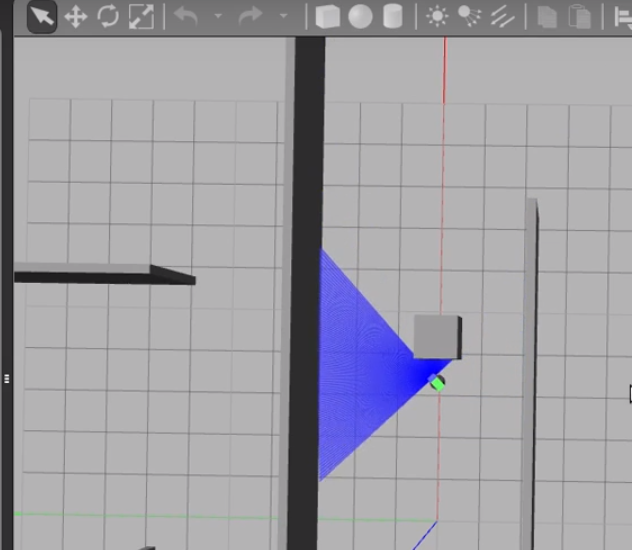
\includegraphics[scale=0.75]{img/robot-example.PNG}
  	\caption{Ejecución del nodo sobre Turtlebot}
  	\label{fig:turtlebot}
\end{figure}


De esta forma, en pocos y sencillos pasos conseguimos programar un robot de forma autónoma para que evite cualquier obstáculo que se encuentre en su camino.


\section{Persecución entre drones}
\label{sec:persecucion-drones}

En este ejemplo por el contrario, como robot final utilizamos un dron, mucho más interesante desde el punto de vista práctico, aunque igual de interesante desde el punto de vista didáctico. Al igual que con la prueba anterior hemos utilizado Gazebo como motor de simulación.\\

El ciclo de vida es el mismo que el que hemos seguido para la ejecución del robot. Primero se genera el proyecto en Scratch, el cual mostramos en la siguiente imagen:\\

\begin{figure}[H]
    \centering
    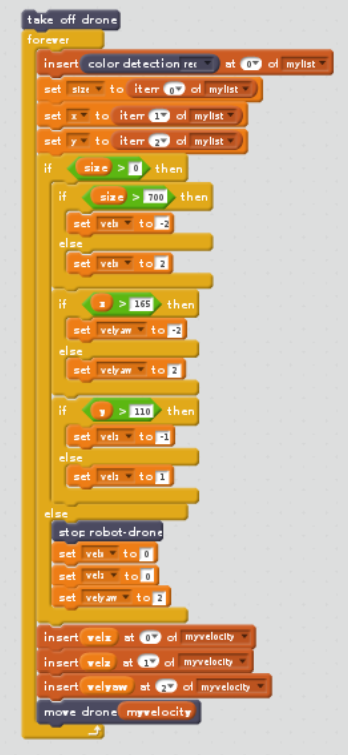
\includegraphics[scale=0.75]{img/cat-drone-scratch.PNG}
  	\caption{Programación en Scratch del drone perseguidor}
  	\label{fig:turtlebot}
\end{figure}

Mediante las funcionalidades que nos aporta ROS para el lanzamiento de aplicaciones bajo un solo comando ejecutamos la traducción, obteniendo nuestro nodo programado en Python. Mostramos el detalle de la traducción de este proyecto, la cual se integrará en el nodo final ROS como hemos descrito en apartados anteriores.

\begin{lstlisting}[language=python,firstnumber=1]
 		mylist = [] 
 		myvelocity = []
        robot.take_off()
        while True:
            mylist.insert(0, robot.color_detection('red'))
            size = mylist[0][0]
            x = mylist[0][1]
            y = mylist[0][2]
            if size > 0: 		 # Tras detectar el objetivo, estima velocidades
                if size > 700:
                    velx = '-2'
                else:
                    velx = '2'
                if x > 165:
                    velyaw = '-2'
                else:
                    velyaw = '2'               
                if y > 110:
                    velz = '-1'
                else:
                    velz = '1'               
            else:			# Gira sobre si mismo buscando el objetivo
                robot.stop()
                velx = '0'
                velz = '0'
                velyaw = '2'            
            myvelocity.insert(0, velx)
            myvelocity.insert(1, velz)
            myvelocity.insert(2, velyaw)
            robot.move_vector(myvelocity)
\end{lstlisting}

Y por último, ya con nuestro nodo generado, agregando la configuración pertinente estará todo listo para su ejecución.

\begin{lstlisting}[language=json,firstnumber=1]
drone:
  Camera:
    Topic: "/solo/cam_frontal/image_raw"
    Name: UAVViewerCamera    
  Pose3D:
    Topic: "/mavros/local_position/odom"
    Name: UAVViewerPose3d
  CMDVel:
    Topic: "/mavros/setpoint_velocity/cmd_vel"
    Name: UAVViewerCMDVel    
  Navdata:
    Topic: "/IntrorobROS/Navdata"
    Name: UAVViewerNavdata 
  Extra:
    TopicArming: "mavros/cmd/arming"
    TopicLand: "mavros/cmd/land"
    TopicSetMode: "mavros/set_mode"
    TopicVel: "/mavros/setpoint_velocity/cmd_vel"
    Name: UAVViewerExtra
NodeName: drone
\end{lstlisting}
Tras ejecutar el nodo junto con el fichero de configuración, obtenemos el resultado deseado, como observamos en la imagen superior. Algo tan complejo como una persecución entre dos drones, totalmente programado en un lenguaje tan simple como Scratch, y esto, es solo una prueba del potencial de esta herramienta.\\


\begin{figure}[H]
    \centering
    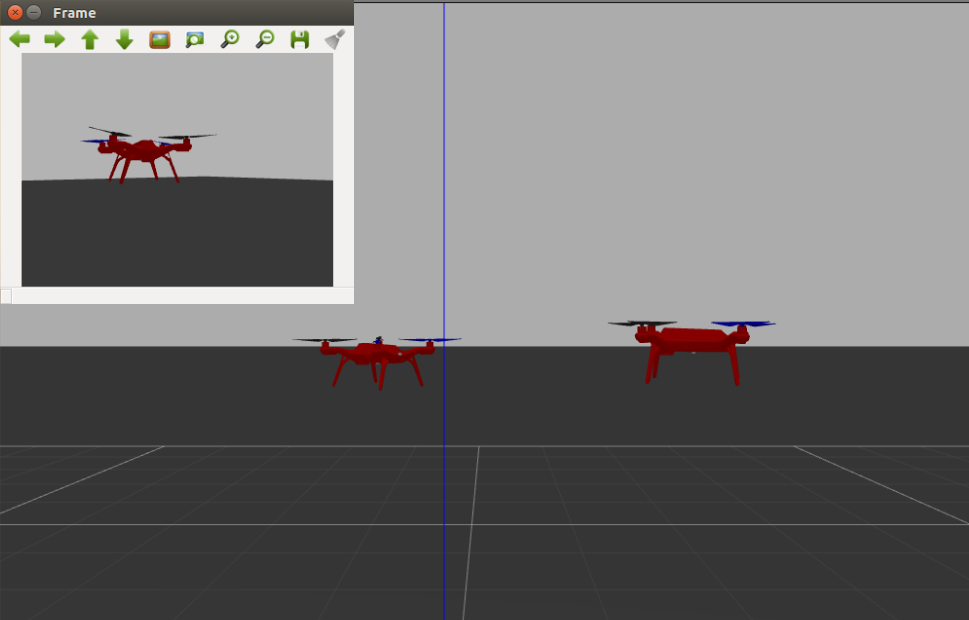
\includegraphics[scale=0.60]{img/drones-fly.PNG}
  	\caption{Ejecución del drone perseguidor}
  	\label{fig:drone-pers}
\end{figure}


Con estos ejemplos hemos recorrido el ciclo de vida de nuestra herramienta, explicando su funcionamiento, además de validar experimentalmente todas las mejoras en el funcionamiento de Scratch4Robots 2.0. Las mejoras en la ejecución de la herramienta mediante simples comandos, sin necesidad de indagar en el código fuente. Y completo funcionamiento de la herramienta, con comunicaciones ROS. 



\cleardoublepage
\chapter{Conclusiones}
Tras detallar en profundidad las mejoras aportadas a la herramienta Scratch4Robots,  este capítulo se ha reservado para ver hasta qué punto se han logrado los objetivos establecidos, para resumir los conocimientos adquiridos durante su desarrollo y para exponer las posibles mejoras que se pueden introducir en trabajos futuros.

\section{Conclusiones}
\label{sec:conclusiones}

El objetivo global de este proyecto era la mejora de la herramienta Scratch4Robots 1.0. Este objetivo se ha alcanzado con éxito a través de una serie de subobjetivos. Estos subobjetivos se dividen en la refactorización de la herramienta, y la extensión en funcionalidad de ésta con el desarrollo de nuevos bloques, una paquetización completa de la herramienta, y la validación experimental con robots ROS.\\

El primer subobjetivo consiste en la refactorización y extensión en funcionalidad. Esto se consigue haciendo modificaciones tanto en el proceso de traducción, en la generación del nodo final ejecutable y en los propios bloques ya existentes en la herramienta. La traducción que aportamos ofrece una mayor capacidad de detección de bloques anidados, además de soportar una mayor cantidad de bloques propios de Scratch. \\

Como parte de esta refactorización, el código generado, ahora es un único nodo ROS programado en Python, con toda la lógica para funcionar de forma autónoma, a este nodo ROS se le aporta la flexibilidad de ser configurado a través de un fichero de configuración, en el que se indican las necesidades de nuestro desarrollo, como pueden ser sensores, actuadores etcétera. \\

Otro de los cambios que aporta esta refactorización es la adaptación a comunicaciones ROS en su totalidad. Se añade el uso de listas para la aceptación parámetros complejos de entrada y salida por parte de los bloques. En cuanto a la extensión de funcionalidades, aportamos nuevos bloques. Como bloque destacado se agrega el bloque perceptivo de detección de objetos de un color determinado, que usa una cámara montada sobre el robot. Se aportan otros bloques de carácter general, como son los bloques matemáticos y lógicos, además de todos los bloques para el manejo de listas. Estos bloques amplían las posibilidades de uso de la herramienta de forma considerable.\\

En segundo lugar se busca una paquetización completa de la herramienta. Esto se consigue de dos formas. La primera y principal, es la generación de un paquete ROS, instalable en forma de binario desde linea de comandos en un sistema operativo Ubuntu. Este paquete además de ser fácilmente instalable, hace uso de todas las funcionalidades que nos aporta el entorno ROS, como por ejemplo la ejecución de nodos pertenecientes a un paquete ya instalado, desde linea de comandos. Esta funcionalidad es en la que nos basamos para lanzar el nodo que realiza la traducción del bloque Scratch al nodo ROS final. Además de esta paquetización ROS, realizamos otra labor de desacople de dependencias en forma de paquetes pip, igualmente instalables desde linea de comandos. Esto aporta una mayor flexibilidad a la herramienta, pudiendo agregar y modificar funcionalidad sin necesidad de modificar el core de la herramienta.\\

Por último queremos hacer una validación experimental de la herramienta con robots puramente ROS. Este subobjetivo se lleva a cabo con la total incorporación de comunicaciones ROS, tanto para Turtlebots como para drones. Estas comunicaciones son validadas con una serie de ejemplos funcionales sobre robots simulados.\\

El objetivo se ha conseguido cumpliendo con los requisitos previos que nos habíamos propuestos. Todo el código se realiza en lenguaje Python. El paquete ROS generado, se trata de un ROS en su versión Kinetic, versión que está enfocada a su uso sobre Ubuntu 16.04, otro de los requisitos que establecíamos. Además no necesitamos de más software, aparte del mencionado anteriormente y el propio Scratch 2.0 en su versión \textit{offline}.


\section{Trabajos Futuros}
\label{sec:trabajos-futuros}

El desarrollo de este trabajo ha generado la versión 2.0 de Scratch4Robots, pero aún quedan muchas cosas que se pueden desarrollar para mejorar la herramienta.\\

El más destacado y de necesaria implementación para que la herramienta se mantenga actualizada, es la integración con Scratch 3.0. Siguiente versión que sale a la luz a principios de 2019. Ayudaría a mantener al día la herramienta con la tecnología del momento. Esto es de vital importancia si buscamos la usabilidad de ésta, una herramienta desactualizada hará que los usuarios se decanten por otras de mayor valor, además de impedirnos el desarrollo de funcionalidades de mayor complejidad por las limitaciones que supone el mantenernos en le versión 2.0 de Scratch. El ser compatibles en un futuro con Scratch 3.0 nos permite crecer tanto cuantitaviamente como cualitativamente, pudiendo ganar más usuarios y además ampliando nuestras funcionalidades, ya que podríamos incorporar funcionalidades como el uso de servicios web que proporciona Scratch 3.0. \\

Otra mejora sería la ampliación de la gama de robots soportados. En esta versión nos hemos centrado en drones y en Turtlebots, pero existe una completa gama de robots de diferentes características a las que podríamos dar soporte. Uno podría ser el robot humanoide Pepper, muy popular actualmente. Esto supondría la generación de bloques para las necesidades específicas de estos robots.\\

De cara a su usabilidad, se podría ampliar el repertorio de tutoriales y guías didácticas. Enfocándolas al aprendizaje de la programación de robots sofisticados para usuarios con un perfil técnico bajo. Esto podríamos acompañarlo con entornos simulados que se descarguen junto con nuestra herramienta, entornos con características suficientes como para poder programar la resolución de desafíos de diversas complejidades, desde Scratch en conjunción con nuestra herramienta.\\

\nocite{*}
\bibliographystyle{unsrt}
\bibliography{Memoria}
\addcontentsline{toc}{chapter}{Bibliografía}

\cleardoublepage
\end{document}
